\documentclass[conference]{IEEEtran}
% by rodolfolabiapari
\usepackage[utf8]{inputenc}
% \usepackage{pdfsync}


\usepackage{tabularx,dcolumn} %tabela
\usepackage{booktabs}
\newcommand{\raaa}[1]{\renewcommand{\arraystretch}{#1}}

\newcommand{\vars}{\texttt}
\newcommand{\func}{\textrm}


% *** CITATION PACKAGES ***
%
\usepackage{cite}
% cite.sty was written by Donald Arseneau
% V1.6 and later of IEEEtran pre-defines the format of the cite.sty package
% \cite{} output to follow that of the IEEE. Loading the cite package will
% result in citation numbers being automatically sorted and properly
% "compressed/ranged". e.g., [1], [9], [2], [7], [5], [6] without using
% cite.sty will become [1], [2], [5]--[7], [9] using cite.sty. cite.sty's
% \cite will automatically add leading space, if needed. Use cite.sty's
% noadjust option (cite.sty V3.8 and later) if you want to turn this off
% such as if a citation ever needs to be enclosed in parenthesis.
% cite.sty is already installed on most LaTeX systems. Be sure and use
% version 5.0 (2009-03-20) and later if using hyperref.sty.
% The latest version can be obtained at:
% http://www.ctan.org/pkg/cite
% The documentation is contained in the cite.sty file itself.






% *** GRAPHICS RELATED PACKAGES ***
%
\ifCLASSINFOpdf
  \usepackage[pdftex]{graphicx}
  % declare the path(s) where your graphic files are
  \graphicspath{{./img/}}
  % and their extensions so you won't have to specify these with
  % every instance of \includegraphics
  \DeclareGraphicsExtensions{.pdf,.jpeg,.png}
\else
  % or other class option (dvipsone, dvipdf, if not using dvips). graphicx
  % will default to the driver specified in the system graphics.cfg if no
  % driver is specified.
  % \usepackage[dvips]{graphicx}
  % declare the path(s) where your graphic files are
  % \graphicspath{{../eps/}}
  % and their extensions so you won't have to specify these with
  % every instance of \includegraphics
  % \DeclareGraphicsExtensions{.eps}
\fi

% *** MATH PACKAGES ***
%
%\usepackage{amsmath}
% A popular package from the American Mathematical Society that provides
% many useful and powerful commands for dealing with mathematics.
%
% Note that the amsmath package sets \interdisplaylinepenalty to 10000
% thus preventing page breaks from occurring within multiline equations. Use:
%\interdisplaylinepenalty=2500
% after loading amsmath to restore such page breaks as IEEEtran.cls normally
% does. amsmath.sty is already installed on most LaTeX systems. The latest
% version and documentation can be obtained at:
% http://www.ctan.org/pkg/amsmath


% *** SPECIALIZED LIST PACKAGES ***
%
%\usepackage{algorithmic}
% algorithmic.sty was written by Peter Williams and Rogerio Brito.
% This package provides an algorithmic environment fo describing algorithms.
% You can use the algorithmic environment in-text or within a figure
% environment to provide for a floating algorithm. Do NOT use the algorithm
% floating environment provided by algorithm.sty (by the same authors) or
% algorithm2e.sty (by Christophe Fiorio) as the IEEE does not use dedicated
% algorithm float types and packages that provide these will not provide
% correct IEEE style captions. The latest version and documentation of
% algorithmic.sty can be obtained at:
% http://www.ctan.org/pkg/algorithms
% Also of interest may be the (relatively newer and more customizable)
% algorithmicx.sty package by Szasz Janos:
% http://www.ctan.org/pkg/algorithmicx


% *** ALIGNMENT PACKAGES ***
%
%\usepackage{array}
% Frank Mittelbach's and David Carlisle's array.sty patches and improves
% the standard LaTeX2e array and tabular environments to provide better
% appearance and additional user controls. As the default LaTeX2e table
% generation code is lacking to the point of almost being broken with
% respect to the quality of the end results, all users are strongly
% advised to use an enhanced (at the very least that provided by array.sty)
% set of table tools. array.sty is already installed on most systems. The
% latest version and documentation can be obtained at:
% http://www.ctan.org/pkg/array


% IEEEtran contains the IEEEeqnarray family of commands that can be used to
% generate multiline equations as well as matrices, tables, etc., of high
% quality.




% *** SUBFIGURE PACKAGES ***
%\ifCLASSOPTIONcompsoc
%  \usepackage[caption=false,font=normalsize,labelfont=sf,textfont=sf]{subfig}
%\else
%  \usepackage[caption=false,font=footnotesize]{subfig}
%\fi
% subfig.sty, written by Steven Douglas Cochran, is the modern replacement
% for subfigure.sty, the latter of which is no longer maintained and is
% incompatible with some LaTeX packages including fixltx2e. However,
% subfig.sty requires and automatically loads Axel Sommerfeldt's caption.sty
% which will override IEEEtran.cls' handling of captions and this will result
% in non-IEEE style figure/table captions. To prevent this problem, be sure
% and invoke subfig.sty's "caption=false" package option (available since
% subfig.sty version 1.3, 2005/06/28) as this is will preserve IEEEtran.cls
% handling of captions.
% Note that the Computer Society format requires a larger sans serif font
% than the serif footnote size font used in traditional IEEE formatting
% and thus the need to invoke different subfig.sty package options depending
% on whether compsoc mode has been enabled.
%
% The latest version and documentation of subfig.sty can be obtained at:
% http://www.ctan.org/pkg/subfig




% *** FLOAT PACKAGES ***
%
%\usepackage{fixltx2e}
% fixltx2e, the successor to the earlier fix2col.sty, was written by
% Frank Mittelbach and David Carlisle. This package corrects a few problems
% in the LaTeX2e kernel, the most notable of which is that in current
% LaTeX2e releases, the ordering of single and double column floats is not
% guaranteed to be preserved. Thus, an unpatched LaTeX2e can allow a
% single column figure to be placed prior to an earlier double column
% figure.
% Be aware that LaTeX2e kernels dated 2015 and later have fixltx2e.sty's
% corrections already built into the system in which case a warning will
% be issued if an attempt is made to load fixltx2e.sty as it is no longer
% needed.
% The latest version and documentation can be found at:
% http://www.ctan.org/pkg/fixltx2e


%\usepackage{stfloats}
% stfloats.sty was written by Sigitas Tolusis. This package gives LaTeX2e
% the ability to do double column floats at the bottom of the page as well
% as the top. (e.g., "\begin{figure*}[!b]" is not normally possible in
% LaTeX2e). It also provides a command:
%\fnbelowfloat
% to enable the placement of footnotes below bottom floats (the standard
% LaTeX2e kernel puts them above bottom floats). This is an invasive package
% which rewrites many portions of the LaTeX2e float routines. It may not work
% with other packages that modify the LaTeX2e float routines. The latest
% version and documentation can be obtained at:
% http://www.ctan.org/pkg/stfloats
% Do not use the stfloats baselinefloat ability as the IEEE does not allow
% \baselineskip to stretch. Authors submitting work to the IEEE should note
% that the IEEE rarely uses double column equations and that authors should try
% to avoid such use. Do not be tempted to use the cuted.sty or midfloat.sty
% packages (also by Sigitas Tolusis) as the IEEE does not format its papers in
% such ways.
% Do not attempt to use stfloats with fixltx2e as they are incompatible.
% Instead, use Morten Hogholm'a dblfloatfix which combines the features
% of both fixltx2e and stfloats:
%
% \usepackage{dblfloatfix}
% The latest version can be found at:
% http://www.ctan.org/pkg/dblfloatfix




% *** PDF, URL AND HYPERLINK PACKAGES ***
%
\usepackage{url}
% url.sty was written by Donald Arseneau. It provides better support for
% handling and breaking URLs. url.sty is already installed on most LaTeX
% systems. The latest version and documentation can be obtained at:
% http://www.ctan.org/pkg/url
% Basically, \url{my_url_here}.




% *** Do not adjust lengths that control margins, column widths, etc. ***
% *** Do not use packages that alter fonts (such as pslatex).         ***
% There should be no need to do such things with IEEEtran.cls V1.6 and later.
% (Unless specifically asked to do so by the journal or conference you plan
% to submit to, of course. )


% correct bad hyphenation here
\hyphenation{op-tical net-works semi-conduc-tor}

% !TEX root = ../main.tex
% !TeX encoding = UTF-8
\usepackage{verbatim}
\usepackage[brazilian]{babel}
\usepackage[utf8]{inputenc}
\usepackage{todonotes}
\usepackage{amssymb}
\usepackage{amsmath}
\usepackage{amstext}
\usepackage{amscd}
\usepackage{amsthm}
\usepackage[algoruled,linesnumbered,lined,portuguese]{algorithm2e}


\newcommand{\hardware }{\textit{hardware}}
\newcommand{\Hardware }{\textit{Hardware}}
\newcommand{\software }{\textit{software}}
\newcommand{\Software }{\textit{Software}}
\newcommand{\hardwares}{\textit{hardwares}}
\newcommand{\Hardwares}{\textit{Hardwares}}
\newcommand{\softwares}{\textit{softwares}}
\newcommand{\Softwares}{\textit{Softwares}}

\newcommand{\hs}{\textit{hardware}\ e\ \textit{software}}
\newcommand{\HS}{\textit{Hardware}\ e\ \textit{Software}}

\newcommand{\wearable} {\textit{wearable}}
\newcommand{\Wearable} {\textit{Wearable}}
\newcommand{\wearables}{\textit{wearables}}
\newcommand{\Wearables}{\textit{Wearables}}


\newcommand{\buffer}   {\textit{buffer}}
\newcommand{\design}   {\textit{design}}
\newcommand{\designer} {\textit{designer}}
\newcommand{\Design}   {\textit{Design}}
\newcommand{\Designer} {\textit{Designer}}
\newcommand{\designs}  {\textit{designs}}
\newcommand{\designers}{\textit{designsers}}
\newcommand{\Designs}  {\textit{Designs}}
\newcommand{\Designers}{\textit{Designers}}
\newcommand{\assembly} {\textit{assembly}}
\newcommand{\profile}  {\textit{profile}}
\newcommand{\Profile}  {\textit{Profile}}
\newcommand{\speedup}  {\textit{speedup}}
\newcommand{\Speedup}  {\textit{Speedup}}
\newcommand{\core}     {\textit{core}}
\newcommand{\cores}    {\textit{cores}}
\newcommand{\codesign} {\textit{codesign}}
\newcommand{\mobile}   {\textit{mobile}}
\newcommand{\benchmark}   {\textit{benchmark}}
\newcommand{\benchmarks}   {\textit{benchmarks}}
\newcommand{\Benchmark}   {\textit{Benchmark}}
\newcommand{\Benchmarks}   {\textit{Benchmarks}}
\newcommand{\titulo}{Uma Abordagem do Problema de Particionamento \Hardware\ e \Software\ para \Design\ de Sistemas Computacionais \Wearables}

\newcommand{\A}{$\mathcal{A}$}
\newcommand{\B}{$\mathcal{B}$}
\newcommand{\C}{$\mathcal{C}$}

%Hyphenations
\hyphenation{XHSTT}
%\hyphenation{res-tri-ções}
\hyphenation{co-nhe-ci-do}
\hyphenation{co-nhe-ci-da}
\hyphenation{re-a-li-za}
\hyphenation{vi-zi-nho}
\hyphenation{clim-bing}
\hyphenation{ran-king}
\hyphenation{me-lhor}
\hyphenation{ou-tras}
\hyphenation{ge-ra-das}
\hyphenation{ex-pe-ri-men-tos}
\hyphenation{pro-ble-ma}
%\hyphenation{su-ges-tões}
\hyphenation{pos-te-rior-men-te}


\begin{document}
%
% paper title
% Titles are generally capitalized except for words such as a, an, and, as,
% at, but, by, for, in, nor, of, on, or, the, to and up, which are usually
% not capitalized unless they are the first or last word of the title.
% Linebreaks \\ can be used within to get better formatting as desired.
% Do not put math or special symbols in the title.
%\title{Uma Abordagem do Problema do Particionamento \Hardware\ e \Software\ para \Design\ de Sistemas Computacionais \Wearables\ com Recursos de \Hardware\ Reconfigurável Limitados}
\title{NÃO UTILIZARUma Abordagem de Particionamento \Hardware\ e \Software\ para \Design\ de \Wearables\ com Recursos de \Hardware\ Reconfigurável Limitados}


% author names and affiliations
% use a multiple column layout for up to three different
% affiliations
\author{
\IEEEauthorblockN{Rodolfo Labiapari Mansur Guimarães}
\IEEEauthorblockA{Departamento de Ciência da Computação\\
Universidade Federal de Ouro Preto\\
Ouro Preto, Brasil 35400--000\\
E-mail: rodolfolabiapari@decom.ufop.br}
\and
\IEEEauthorblockN{Dr. Ricardo Augusto Rabelo Oliveira}
\IEEEauthorblockA{Departamento de Ciência da Computação\\
Universidade Federal de Ouro Preto\\
Ouro Preto, Brasil 35400--000\\
E-mail: rrabelo@gmail.com}}

% conference papers do not typically use \thanks and this command
% is locked out in conference mode. If really needed, such as for
% the acknowledgment of grants, issue a \IEEEoverridecommandlockouts
% after \documentclass


% use for special paper notices
%\IEEEspecialpapernotice{(Invited Paper)}


% make the title area
\maketitle

% As a general rule, do not put math, special symbols or citations
% in the abstract
\begin{abstract}
Este constitui-se de uma abordagem do problema de particionamento \hs\ para dispositivos \wearables com foco em aumento de performance, visando o gasto de recursos em seu \textit{trade-off}.
A tecnologia de fatores como microeletrônica, sensores e comunicação móvel são constantemente melhoradas à medida que a informação também torna-se mais necessária, tornando-a um estímulo para o desenvolvimento de dispositivos inteligentes e conectados como sistemas embarcados, IoTs ou \wearables.
Isso é visto no rápido desenvolvimento de dispositivos para comércio, entretanto, ainda com a dificuldade de satisfazer os requisitos das várias aplicações modernas.
Tais dispositivos utilizam de um leque de sensores e necessitam de um serviço autônomo, o que implica numa demanda de performance somado com o baixo consumo de energia sem deixar \design, segurança e confiabilidade a desejar.
Para obter um produto de alta qualidade, atendendo aos requisitos, este consiste na análise de projetos para \wearables\ utilizando plataformas FPGA como meio na realização de particionamentos \hs\ obtendo \speedup\ e eficiência em comparação a outros sistemas como \textit{in-software}.

Palavras-chave: Particionamento \hs, Sistema \Wearable, Sistemas Embarcados.
\end{abstract}

% no keywords




% For peer review papers, you can put extra information on the cover
% page as needed:
% \ifCLASSOPTIONpeerreview
% \begin{center} \bfseries EDICS Category: 3-BBND \end{center}
% \fi
%
% For peerreview papers, this IEEEtran command inserts a page break and
% creates the second title. It will be ignored for other modes.
\IEEEpeerreviewmaketitle
a
%% !TEX root = ../main.tex
% !TeX encoding = UTF-8
\section{Introdução} \label{chap:introducao}

   %\todo[inline]{contextualização lógica}
	%intro geralzona
	O recente progresso na obtenção e manipulação de informações, em conjunto com a ascensão da tecnologia microeletrônica, comunicação e sensores, proporcionou estímulos no desenvolvimento de sistemas computacionais inteligentes de comunicação e \wearables, todos sendo dispositivos embarcados \cite{Jozwiak2017}.
	%
	%O projeto de sistemas computacionais está mais complexo que nunca. A demanda por curto tempo para disponibilidade ao mercado, somado ao fato dos produtos exigirem propriedades de corretude, rapidez, confiabilidade e preço acessível, representam um desafio para projetistas de sistemas embarcados em geral.
	%Sistemas computacionais embarcados (também nomeados como sistemas embarcados ou sistemas embutidos) possuem muitos componentes implementados tanto em \hs, e esta decisão de implementação será o tema principal abordado nesta pesquisa com foco em dispositivos \wearable.

	% embedded
   %\todo[inline]{A parte de wearable vc tem q explorar mais no capitulo 1 tb, como construcao da motivacao. Uma introducao tem q ser a sequinte sequencia}
	Os sistemas embutidos são produtos que utilizam processadores/controladores e podem estar desde fornos de microondas, até sistemas de controle de aeronaves.
   São computadores situados em dispositivos e que sua presença não é imediatamente óbvia \cite{Wolf1994}.
	%Requerem técnicas na qual difere das utilizadas para \design\ de computadores de propósito geral ou aplicações de \software\ dessas máquinas \cite{Wolf1994}.
	%Em 2015, foi previsto um total de 6,5 bilhões de dispositivos ativamente conectados para o ano de 2016, segundo notícias da empresa de pesquisa e consultoria Gartner \cite{RobvanderMeulen2015}.

	% wearable
	Ainda neste âmbito, existe um subconjunto na qual possui o propósito de integrar-se ao sistema corporal expandindo suas capacidades, onde, diferentemente de \textit{smartphones} e \textit{tablets}, cria-se uma integração cada vez mais intensa entre tecnologia e ser humano.
	Chamados de sistemas \wearables, são requeridos para prover serviço autônomo, contínuo, em um longo período de tempo.
   %Sua tendência é superar os dispositivos manuais como computadores e telefones pois são dispositivos mais sofisticados pela existência de recursos sensoreais e escaneamento.
   %
   %Cerca de 20\% da população possui pelo menos um dispositivo sendo que 10\% utiliza-o todos os dias \cite{lee2016information}.
   %São dispositivos que permitem benefícios como um estilo de vida inspirado em dados \textit{fitness} até realidade aumentada preenchida por objetos virtuais.
	%Tais dispositivos demandam de uma alta performance e/ou baixo consumo de energia, sem apresentar \textit{trade-off} de confiabilidade e segurança entre outros. % \cite{Jozwiak2017}.
	%
	%Segundo o trabalho de \cite{Jozwiak2017}, com computação de alta performance e estudos em gasto energético eficiente, foi possível a facilitação do rápido progresso da computação móvel e autônoma.
	%Tudo isso deve-se à possibilidade de comunicar-se com a rede global de comunicação, combinada com o progresso de sensores e atuadores, criando novas oportunidades importantes de projeto.
	%%Exemplos disso são indústrias inteligentes, cidades e casas, bem como setores de IoT, sistemas móveis como automóveis inteligentes, computação móvel como \textit{smartphones}, comunicação e, não menos importante, os sistemas computacionais \wearable.
	\Wearables\ podem ser definidos como `embutidos que foram inseridos em ambiente \mobile\ de seus usuários, não exercendo a mesma atividade' e seu propósito é criar dispositivos com acesso constante, conveniente, portátil e principalmente \textit{hands-free}, aplicando não só na área de saúde e esportiva, mas também em entretenimento e assim por diante.

   %\todo[inline]{1- Apresnetar o problema:}
   \subsection{Problema}
   	% intro particionamento
   	A redução do ciclo de comercialização de um produto e o aumento de sua eficiência de desenvolvimento de projeto tem se tornado uma preocupação na área de \design\ de sistemas.
   	Com isso, o particionamento \hs\ tem sido um dos métodos tecnológicos para o desenvolvimento de sistemas embarcados em geral, já que, este afeta a performance do sistema como um todo \cite{Hassine2017}.
      Visa o balanceamento de todas as tarefas de forma a otimizar alguns objetivos sistêmicos sobre determinadas restrições \cite{Hidalgo1997}.
   	Segundo \cite{Wolf1994, Edwards1994}, sistemas embutidos gerais são considerados únicos pelo fato da necessidade de um \codesign\ de \hs, e suas pesquisas têm como objetivo o \design\ de sistemas heterogêneos, visando performance, custo e metas de confiabilidade.

      %Os grupos designados ao \software\ são executados sequencialmente pelo respectivo processador do sistema enquanto os mapeados em \hardware\ são implementados por uma combinação customizada ou por circuitos sequenciais \cite{Sass2010}.

   	% particionamento
   	%Quando necessita de performance ao realizar o \codesign\ (termo referente ao inglês \textit{Participatory Design}) de \hs\ para sistemas embutidos, o problema de qual função do sistema deverá ser implementada em \hardware\ ou em \software\ emerge e esse problema é conhecido por particionamento \hs\ (\textit{hardware/software partitioning}).
   	%Um significante esforço foi posto nesta área nos últimos dez anos, segundo \cite{Trindade2016}.

      %Um desafio de \design\ é combinar a flexibilidade de demanda pelos vários ambientes e aplicações, e a alta performance exigida em tarefas com o baixo consumo de energia requerido para maximizar o tempo de uso da bateria.

      %\todo[inline]{3- Motivacao pra resolver este problema:}

   	%Com o desenvolvimento de sistemas embutidos cada vez mais complexos, o particionamento \hs\ tornou-se um problema de otimização em \codesign\ de sistemas \cite{Yan2017}.
      %A motivação é que, tal problema que envolve \design\ colaborativo e multidisciplinar, é um passo-chave no \design\ de produtos modernos \cite{Trappey2016}.
      %Implementações que baseiam-se somente em módulos de \software\ possuem mais flexibilidade e menos custosos, entretanto, seu custo eleva-se em termos de tempo de execução.
      Uma implementação de \hardware\ customizada de um conjunto de computações proverá uma eficiência energética e \speedup\ maior relativa à implementações em \software\ \cite{Zhang2008, Hassine2017, Wolf1994, Canis2011, Stone2010}.

      % combinação de fpga com cpu
      A tendência hoje para \design\ é na combinação das funções do processador com os recursos dos arranjo de portas programáveis em campo (FPGAs, do inglês \textit{Field-Programmable Gates Array}) formando um sistema computacional híbrido. %, exemplo exibido na Figura \ref{fig:i-soc}. %\cite{Plessl2003}
      %O conceito de CSoC é importante quando necessita da construção de sistemas computacionais que podem utilizar de circuitos junto à um processador como é o caso de sistemas embutidos.
   	Ao utilizar do FPGA para o problema de particionamento, é possível acelerar uma aplicação usando recursos de \hardware\ melhorando no desempenho e eficiência energética em comparação com o \software\ executado inteiramente em um processador \cite{Cong2009, Lo2009, Zhang2008a}.
      %A Microsoft em \cite{Putnam2014} aceleraram o \textit{Bing Search} em duas vezes com a utilização de FPGAs em seus \textit{data centers} \cite{Putnam2014}.
      %além da aquisição da Altera, uma das duas maiores vendedoras de FPGAS no mundo, pela Intel em \cite{Maan2015} por cerca de $ 16.7 $ bilhões de dólares \cite{Maan2015}.


      %{4- Contribuicao ao resolver o problema:}

      %{5- Objetivos:}

      %Este trabalho então, propõe o estudo e aplicação de técnicas de particionamento dentro do conjunto de aplicações e sistemas \wearables, na qual, possui restrições significativas como bateria, recursos e custo.
   \begin{comment}
   \subsection{Objetivos da Dissertação}
   	Este trabalho tem como objetivo a abordagem do particionamento \hs\ bem como sua importância no mundo de sistemas computacionais embutidos, com foco em sistemas \wearables\ apresentando algumas soluções utilizadas atualmente.

       \begin{itemize}
         %\item Apresentação do tema de projeto de sistemas computacionais \wearable\ por meio do particionamento \hs;
         %\item Apresentação de uma abordagem metodológica criada para o uso ao problema aplicado no contexto desses sistemas \wearables, na qual possuem restrições relacionados ao custo energético e recursos.

            \item Introdução de sistemas computacionais \wearables\ e apresentação do problema de particionamento \hs\ no âmbito de de sistemas computacionais embutidos, com foco em sistemas \wearables;

            \item Apresentação das principais soluções apresentadas ao logo dos anos e as utilizadas atualmente, bem como as ferramentas HLS como LegUp e OpenCL para a geração de sistemas computacionais que usufruem de aceleradores em \hardware.

            \item Exposição da abordagem metodológica a ser utilizada para a procura da solução do problema de particionamento \hs\ apresentado.
       \end{itemize}

      \subsubsection{Justificativa}

         %{2- Justificativa pq eh um problema relevante:}
      	A justificativa para a realização deste é que, além do tema de particionamento ser proposto recentemente, com o desenvolvimento de \designs\ mais complexos, esse problema de decisão torna-se cada vez mais desafiador para os \designers\ de projeto, no qual o grande requisito para eficiência necessariamente segue junto com a alta velocidade de processamento \cite{Trindade2016, Arato2005, Yan2017}.

      	Dessa forma, pesquisá-lo com foco em sistemas \wearables\ torna-o ainda mais necessário pela pouca atenção dada pelo meio científico até o presente momento, como será demonstrado no decorrer do documento, principalmente pelo ampla utilização que este tipo de produto vem ganhando no espaço comercial.


      \subsubsection{Contribuição}
         O trabalho consiste numa busca sobre o aprimoramento de performance de um dispositivo computacional \wearable\ visando os respectivos gastos relativos ao uso de aceleradores em \hardware\ como recursos, gasto energético, área utilizada e outros itens que serão discutidos neste documento.


   \subsection{Organização da Dissertação}
   	Os demais capítulos deste trabalho estão organizados da seguinte forma:
      No Capítulo \ref{chap:revisao_bibliografica} é apresentada uma revisão bibliográfica do problema, abordando alguns métodos de fundamental importância para este trabalho.
      No Capítulo \ref{chap:relacionados} são descritos alguns trabalhos relacionados ao tema abordado.
      Nos Capítulos \ref{chap:design} e \ref{chap:met2} são apresentadas as metodologias, sendo a primeira a exibição do processo de \design\ e a segunda a metodologia proposta.
      %No Capítulo \ref{chap:experimentos} \todo{são?} apresentados os resultados e suas considerações para o problema.
      No Capítulo \ref{chap:conclusao} são apresentadas as conclusões parciais e propostas de trabalhos futuros.
   \end{comment}


%%!TEX root = ../main.tex
% !TeX encoding = UTF-8
\section{Wearables como Sistemas Processados} \label{chap:revisao_bibliografica}

   Aqui será descrito os principais conceitos do trabalho, além de suas tecnologias e metodologias. Ao final será descritos pesquisas relacionadas.

   \subsection{Fundamentação do Conceito Wearable}
      % Introdução histórica e geral
      Sistemas \wearables\ são sistemas que, com a possibilidade de ter um computador acoplado ao corpo, proporciona ao usuário um nível superior de informações contextualizadas dentro de um ambiente interativo \cite{Amorim2017}.

      %Com a tecnologia constantemente melhorando à medida que a informação se torna sem-fio, os avanços demandaram mais fatores móveis e \wearable\ de produtos que possuem acesso à informação.
      %Segundo \cite{Gemperle1998}, um produto que é \wearable, deveria ter sua `\textit{wearability}' sendo este definido como a interação entre o corpo humano e o objeto \textit{wearable} estendendo ao corpo em movimento.

      Devido ao movimento de seus usuários, um controlador \wearable\ é embutido em um ambiente \mobile\ e necessita-se da interação com o ambiente ao seu redor.
      Com a distribuição espacial dos módulos pelo corpo, a comunicação torna-se um item importante em termos consumo de energia e com isso,
      %A rede de comunicação é uma mistura de conexões cabeadas e sem-fios.
      a comunicação sem-fio é a tecnologia predominante por causa da necessidade de mobilidade e gasto consciente \cite{Plessl2003, Kymissis1998}.



      %wearable precisa ser pequeno
      A introdução desses no ambiente de científico não é nova como é reportado por \cite{Sutherland1968, Mann1996, Mann1997}.
      Entretanto, a aplicação desses dispositivos, depende diretamente da miniaturização dos componentes eletrônicos.
      %aparicão nos dias atuais
      %Esse fenômeno fica claro ao perceber o crescente espaço ganho pelos \textit{smartwatches}, \textit{fitness trackers}, óculos, equipamentos de realidade virtual e aumentada e muitos outros equipamentos embarcados nas atividades pessoais de usuários.
      %Com esses novos dispositivos embarcados de propósito geral miniaturizados, aumenta-se a sua atração devido à fácil disponibilidade dos dispositivos, baixo preço e ferramentas de desenvolvimento disponíveis para desenvolvimento de aplicações específicas incluindo compiladores e sistemas operacionais para tal, mas não são otimizados para uso \wearable.
      %Segundo \cite{Plessl2003}, muitos dos sistemas \wearables\ construídos possuíam características diferentes de componentes que prestam auxílio à tarefas pessoais de usuários com base no paradigma de operações \textit{hands-free} e a propriedade de computação \wearable\ discreta.
      %Sistemas de computação distribuídos no corpo construídos a partir desses equipamentos interativos são altamente ineficientes devido à falta de especialização de componentes individuais de propósito específico.

      Segundo \cite{Hennessy2011}, por mais que exista um leque de processadores para sistemas embutidos, o preço é um dos fatores mais importantes para seu \design, sendo tão importante quanto o requisito de desempenho pois, necessita-se de um desempenho elevado a um preço reduzido.

      Esses dispositivos embarcados podem também trabalhar de forma colaborativa com \textit{smartphones}, redes e outros sistemas criando um sistema mais complexo \cite{Jozwiak2017}.

      A utilização de \hardware\ reconfigurável nos permite alcançar alto poder de processamento com eficiência energética em relação à processadores para tarefas de computação intensiva em tempo real, por exemplo \cite{Plessl2003}.


   \subsection{\textit{Field-Programmable Logic Device} (FPGA)}
      % uso de fpga no mundo
      %Até recentemente, os \hardwares\ reconfiguráveis eram utilizados unicamente na protitipação de projetos de circuitos integrados de aplicação especifica (ASIC, do inglês \textit{application-specific integrated circuit} e produção em baixo volume por causa de sua baixa velocidade e custo por unidade.
      %Entretanto, com a variedade desses dispositivos disponibilizados hoje no mercado, em conjunto com a elevação do custo de engenharia não recorrente (NRE, do inglês \textit{Nonrecurring Engineering}, que refere-se ao custo de pesquisa, \design, desenvolvimento e teste de um novo produto e exigências de mercado), houve um crescente interesse na utilização de FPGAs para sistemas embutidos devido suas vantagens sobre ASICs em termos de flexibilidade de projeto e custo zero de engenharia não recorrente citada \cite{Mei2000}.
      %lousa branca
      %Tais dispositivos, juntos com sua plataforma de interação, de forma geral, permitem ao \designer\ de sistemas embutidos ter uma \textit{lousa branca} em que possa implementar \hardwares\ computacionais personalizados tão facilmente como o desenvolvimento de um \software, como foi possível ilustrar na Figura \ref{fig:rt-board}.

      % Plataforma FPGA
      Uma \textit{plataforma FPGA} é um chip na qual, além de conter o componente FPGA, está integrado à inúmeras interfaces e componentes e seus respectivos circuitos.
      Como possui recursos suficientes para a sintetização de circuitos complexos, é possível implementar inúmeros projetos digitais como funções de processamento de imagem, algoritmos de redes de computadores, criptográficos e \textit{soft}-processadores completos, cada projeto de acordo com os recursos disponíveis \cite{Plessl2003}.
      %Entretanto, enquanto configurar um \hardware\ reconfigurável é uma tarefa fácil graças às ferramentas disponíveis hoje, criar um \design\ de \hardware\ inicial não é \cite{Sass2010}.

      %\begin{figure}[h] \centering
      %   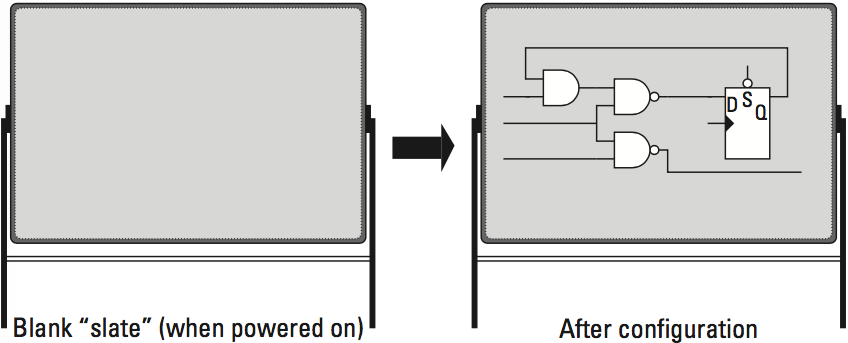
\includegraphics[width=0.75\textwidth]{img/rt-board.png}
      %   \caption{Ilustração em alto nível do funcionamento interno do FPGA. Fonte: \cite{Sass2010}.}
      %   \label{fig:rt-board}
      %\end{figure}

      %A seguir, será descrito a tecnologia que consiste os \hardwares\ reconfiguráveis, em especial o FPGA, e as respectivas linguagens de descrição de \hardware.

   %\subsection{Sua Tecnologia}
      % PLD
      %Para introduzir alguns conceitos, é importante destacar o que são os dispositivos lógicos programáveis (PLDs, do inglês \textit{Programable Logic Devices}).
      %Às vezes chamados de dispositivos lógico programáveis em campo (FPLD, do inglês \textit{Field-Programmable Logic Device}), podem ser adaptados para criar muitos dispositivos digitais, desde simples portas lógicas até estruturas complexas.
      %\cite{tocci2003sistemas, Plessl2003} dizem que com um investimento de capital pequeno, qualquer empresa pode comprar os \softwares\ de desenvolvimento e \hardware\ necessário para programar PLDs para seus projetos digitais.
      %De modo geral, os PLDs são descritos como pertencendo a três tipo diferentes sendo eles os dispositivos lógicos programáveis simples (SPLD), dispositivos lógicos programáveis complexos (CPLDs, do inglês \textit{Complex Programmable Logic Devices}) e arranjo de portas programáveis em campo (FPGA) sendo o último tipo abordado neste trabalho \cite{Brown1996}.

      %LUTS
      O FPGA segundo \cite{tocci2003sistemas}, constitui-se de vários módulos lógicos programáveis, relativamente pequenos, independentes e interconectados, para criar funções maiores.
      %Cada módulo lida, normalmente, com até quatro ou cinco variáveis de entrada.
      %A maioria dos FPGAs utilizam uma \textit{look-up table} (LUT) para criar as funções lógicas desejadas.
      %Uma LUT funciona como uma tabela-verdade, no sentido que a saída é programada para criar a função combinacional armazenando valores verdadeiros e falsos adequado a cada combinação de entrada.
      Os recursos de roteamento de sinal programável dentro do chip tendem a ser bem variados, com extensões de caminhos diferentes disponíveis, adequando a cada sintetização.
      %Os atrasos de sinal em um projeto dependem do roteamento real de sinal selecionado pelo \software\ de programação.
      %Os módulos lógicos também contêm registradores programáveis.
      Eles não são associados a nenhum pino de entrada e saída (I/O, do inglês \textit{Input and Output}).
      Em vez disso, cada pino de I/O é conectado ao bloco programável de entrada e saída que, por sua vez, é conectado aos módulos lógicos com linhas de roteamento selecionadas.

      %\begin{figure}[!t] \centering
      %   \vspace{-10pt}
      %   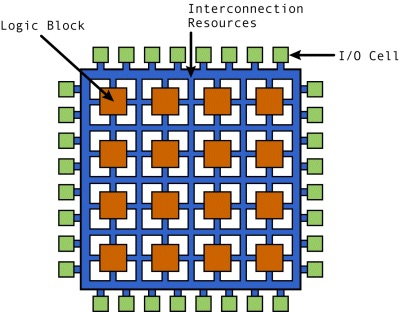
\includegraphics[width=0.5\textwidth]{img/rt-arch_fpga.jpg}
      %   \vspace{-15pt}
      %   \caption{Exemplo da arquitetura internas de um FPGA. Fonte: \url{http://www.eetimes.com/document.asp?doc_id=1274496}. Acesso: 30/05/2017.}
      %   \label{fig:rb-arch_fpga}
      %\end{figure}

      %Uma arquitetura geral simplista de FPGA é exibido na Figura~\ref{fig:rb-arch_fpga}.
      %Nela os quadrados menores situado nas laterais são blocos de I/O que podem ser configurados para fornecer recursos de entrada, saída ou bidirecionais.
      %Os quadrados maiores situados no interior são as LUTs, usados para guardar dados que entram ou saem e realizar as operações lógicas.
      %Os canais que interligam os blocos entre si são estabelecidas por meio de conexões que passam pelas linhas e colunas nos canais entre esses blocos e possuem a funcionalidade de serem interconexões programáveis \cite{tocci2003sistemas}.
      %A tecnologia interna de um FPGA consiste basicamente de um arranjo de blocos lógicos, canais de roteamento para interconexão de blocos lógicos e blocos de entrada e saída de sinais em torno do circuito.
      %FPGAs baseado em SRAM (do inglês \textit{Static Random Access Memory}) utilizam células SRAM para controlar a funcionalidade de blocos lógicos e entrada e saída de sinais bem como as rotas, e pode ser reprogramado arbitrariamente em nível de circuito, muitas vezes, baixando um novo \textit{stream} de dados de configuração para o dispositivo.
      Esses dispositivos possuem milhões de portas de lógicas programáveis, bilhões de transistores, além de outros blocos de \hardware\ dedicados como memórias embarcadas e multiplicadores de ponto-fixo tornando-os um dos circuitos integrados (CI) mais densos existente \cite{Choi2016}.

      % tecnologia e energia
      Segundo \cite{tocci2003sistemas},
      %tais maravilhas de flexibilidade de projetos digital podem fornecer uma série de opções de projeto sendo voltados para indústria e até mesmo educação.
      ao utilizar tecnologia CMOS, o consumo de energia do chip é relativamente baixo comparado com outras tecnologias podendo ser confeccionado em nível de tensão elétrica, frequências e cargas para os sinais de I/O.
      %O mercado fornece diferentes graus de velocidade de FPGA a fim de que o projetista utilize o mais adequado ao projeto.
      %Entretanto, um dispositivo FPGA pode ser configurado para um número infinito de projetos e isso implica na não possibilidade de afirmar o montante de dissipação de energia para um dispositivo FPGA.
      %O \software\ Quartus II tem duas ferramentas para estimular o montante de uso de energia para uma aplicação.
      %O \textit{PowerPlay Early Power Estimator} é usado durante os estágios iniciais do projeto para estimar a magnitude de potência do dispositivo.
      Dessa forma, FPGAs são chips que podem ser programados instantaneamente para funções de qualquer circuito digital \cite{Choi2016}.

      % Importancia
      %\cite{tocci2003sistemas, Plessl2003} citam ainda que o motivo de PLDs estarem dominando o mercado é o fato de que, como são dispositivos programáveis, a mesma funcionalidade pode ser obtida com um circuito integrado (CI) ao invés de diversos circuitos individuais.
      Isso significa maior confiabilidade, menor espaço ocupado na placa, consumo de energia, complexidade de desenvolvimento e, geralmente, menor custo de fabricação.

      \subsubsection{\textit{Hard} e \textit{Software Cores}}
         % Utilização de um processador sintético ou físico
         A unidade de processamento central (CPU, do inglês \textit{Central Processing Unit}) nesses tipos de sistema pode estar disposta em duas naturezas distintas, sendo estas \textit{hard} e \textit{soft} \cores.
         A primeira é um \core\ dedicado, ou seja, um pedaço de circuito integrado dentro (ou não) de um FPGA, enquanto a segunda é feita por meio da sintetização de um processador no FPGA utilizando seus recursos lógicos, ou seja, \design\ e sintetização na placa.
         Independente de sua natureza, o sistema, cujo nome torna-se SoC FPGA (do inglês, \textit{System-on-Chip} FPGA), terá a seguinte arquitetura exibida na Figura~\ref{fig:rb-soc}.
         
         \begin{figure}[h] 
            \centering
            \vspace{-1em}
            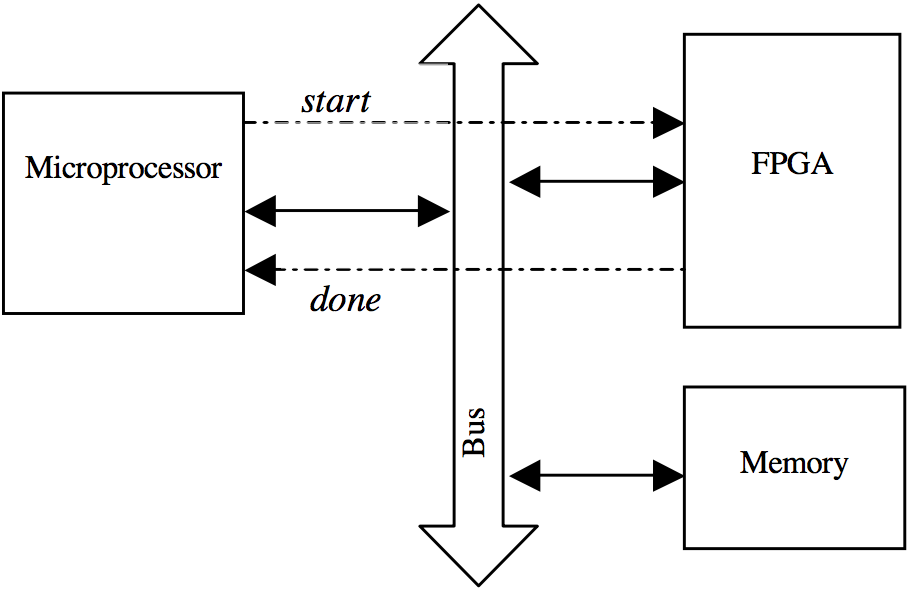
\includegraphics[width=0.35\textwidth]{img/into-soc.png}
            \caption{Visão geral de um SoC FPGA. As setas representam os barramentos de comunicação entre os principais componentes.}
            \label{fig:rb-soc}
         \end{figure}
         
         Cada um tipo de \core\ possui suas vantagens.
         Ao utilizar um \textit{hard} \core, é possível utilizar todos seus recursos obtendo máxima performance nas atividades executadas, a utilização de um \textit{soft} \core\ permite a extensão/configuração de sua arquitetura \cite{Plessl2003}.

         %Um das maiores barreiras para o \design\ de projetos em FPGA é a necessidade de uso de linguagens de descrição de \hardware.
         %Elas serão descritas a seguir.

   \subsection{Profiling} \label{sec:profile}
         \Profile\ é uma procedimento para auxiliar o desenvolvedor a coletar informações do \software\ em tempo de execução.

         O processo é feito ao colocar o \software\ referencial (programa a ser analisado) como entrada representativa na ferramenta e a coleta é realizada em várias partes da aplicação ao longo de sua execução neste.
         Uma das técnicas do \profile\ de mensurar uma aplicação é na realização de interrupções periódica no programa e amostrar o seu \textit{program counter}.
         Dessa forma, é possível utilizar um histograma para contar quando um programa é interrompido em um endereço particular e a partir dessa informação, calcular a fração aproximada do tempo total de execução gasto em suas partes \cite{Graham1982}.
         %Distribuições GNU/Linux possuem a ferramenta \texttt{gprof} na qual avalia procedimentos enviados por parâmetro, realizando o cálculo de tais informações de \software\ \cite{Graham1982}.


%%!TEX root = ../main.tex
% !TeX encoding = UTF-8
\subsection{Trabalhos Relacionados}  \label{chap:relacionados}
   % Embedded
   O desenvolvimento com foco em sistemas embutidos ou microcontroladores já é pesquisado amplamente como os trabalhos de \cite{Ernst1993, Gupta1995, Hardt1995, Gajski1994, Bolsens1997}, publicados na década de 90.

   O autor, \cite{Mei2000}, além do particionamento, descreve uma abordagem de escalonamento para sistemas embutidos dinamicamente reconfiguráveis (DRESs, do inglês \textit{dynamically reconfigurable embedded systems}). % no qual possuem como projeto um processador de propósito geral junto com um FPGA sendo este reconfigurável em tempo de execução para reduzir custos.
   Realiza-se análise de tempo de configuração e, como contribuição, a análise do tempo de reconfiguração parcial do FPGA.
   %Com a adição da reconfiguração parcial de \hardware, o escalonamento no FPGA torna-se um problema de alocação restrita, enquanto o escalonamento em circuitos integrados de aplicação específica (ASICs, do inglês \textit{application-specific integrated circuits}) é um problema de serialização.
   %Para o escalonamento, utiliza-se um método baseado na heurística do algoritmo genético (GA, do inglês \textit{genetic algorithm}) e num algoritmo de escalonamento de lista com melhorias.
   %O escalonador desenvolvido atua como uma sub-rotina do algoritmo de particionamento.
   %Ele é invocado no passo \textit{evolution} do GA. Além do escalonamento já conhecido em processador e barramento sequenciais determinando a ordem e tempo início de execução, o algoritmo também deve fazer o escalonament no FPGA.
   %Porém, não só determinando o tempo de início da tarefa, mas sim sua posição no FPGA respeitando as restrições de recursos e precedentes, tornando assim o problema uma abordagem ao problema de alocação restrita.

   Já \cite{Arato2003} descreve algumas versões diferentes do problema de particionamento, correspondendo à sistemas de tempo-real e custo restringido respectivamente, fornecendo análise matemática formal para o problema, provando que são problemas $ \mathcal{NP} $-difícil.
   Apresentara uma abordagem baseada na programação linear inteira resolvendo o problema de forma otimizada, mesmo para sistemas de grande porte, além de outra abordagem utilizando a heurística GA na qual encontrar soluções próximas ao ótimo global para sistemas largos.

   O trabalho de \cite{Mann2007} descreve uma primeira tentativa para um algoritmo exato, não heurístico, para o problema de particionamento.
   Utilizam um esquema na qual implementa-se a estratégia \textit{branch-and-bound} como um \textit{framework}, permitindo o incremento de outros algoritmos.
   %Em sua implementação, realizaram várias investigações para incrementar a eficiência do algoritmo, incluindo várias técnicas sendo elas: \textit{lower bounds based on LP-relaxation}, uma mecânica de inferência customizada, condições não-triviais necessárias baseadas num algoritmo \textit{minimum-cut}, e diferentes heurísticas com passos pré-otimizados.
   O algoritmo também pode ser generalizado a fim de incluir mais de uma restrição, podendo também o \designer\ prescreva quais nós devem estar em qual nível de projeto.
   Eles demonstram que o produto pode resolver problemas de particionamento altamente complexos em tempo razoável.
   %Citam ao final que o resultado obtido é em entorno de dez minutos mais rápido que algoritmos exatos anteriores baseados em programação linear inteira para os testes realizados.

   Pesquisas mais recentes como a de \cite{Hassine2017} procuravam aplicar otimizações sobre o tempo de execução e gasto energético para \cores\ baseados em sistemas embarcados por meio de algoritmos de particionamento.
   O algoritmo proposto destina-se a alcançar um particionamento de grafos à procurar o melhor conjunto da relação energia e tempo de execução.
   Testado em comparação com outros algoritmos heurísticos como \textit{Simulated Annealing}, Busca Tabu e Genético, o algoritmo mostra-se ser melhor adequado para aplicações em \cores\ baseados em sistemas embarcados que necessitam do equilíbrio no \textit{tradeoff} de sistemas embarcados.

   Trabalho como de \cite{Trindade2016} utiliza Algoritmo Genético para solucionar o problema de particionamento em sistemas embutidos.
   Em seu trabalho, é proposto novas abordagens usando técnicas de verificação baseadas nas teorias de módulo de satisfação (SMT, do inglês \textit{satisfiability modulo theories}).
   Apresentam um exemplo de particionamento, modelam e solucionam-o usando três diferentes técnicas sendo a principal ideia é aplicar mo método de verificação SMT ao particionamento \hs, e por fim, comparar os resultados com técnicas de otimizações tradicionais como ILP e GA.

   \textit{Surveys} como de \cite{Jozwiak2017} considera vários aspectos de uma aplicação embutida, bem como suas tecnologias de \design\ com foco sistemas móveis modernos e \wearables.
   É citado dois paradigmas de desenvolvimento para sistemas embutidos sobre sistema de multi-processadores heterogêneos sendo eles o paradigma de sistemas \textit{life-inspired} e sistemas \textit{quality-driven}.
   O paradigma de sistemas \textit{life-inspired} especifica princípios básicos, características e organização funcional e estrutural de um sistema embutido por meio da analogia à vida de um organismo inteligente, além de básicas soluções de mecanismos e arquiteturas de sistemas para implementar tais princípios.
   Já o paradigma de sistemas \textit{quality-driven} (ou seja, orientado pela qualidade) torna-se uma segunda solução para o \design\ de dispositivos que necessitam satisfazer as exigências de \textit{real-time}, baixo consumo de energia, entre outros.
   Dessa forma, especifica-se qual a nova qualidade do sistema a ser requeria e como esta meta é obtida.
   %De forma a facilitar a compreensão, \cite{Jozwiak2017} define qualidade de uma solução sistêmica proposto como o total de sua eficácia e eficiência na resolução do problema real.
   %Eficácia entende-se como o grau em que uma solução atinge seus objetivos e a eficiência o grau em que uma solução usa recursos para realizar seus objetivos e juntas determinam o grau de excelência.
   %Elas são expressas em termos de parâmetros mensuráveis, o que é necessário para implementar o design \textit{quality-driven}.
   Entretanto, é descrito ao final que, enquanto \designers\ aprenderam bastante na construção de plataformas de \hardware\ heterogêneos altamente paralelos, os métodos e ferramentas automatizadas para a sua programação e o paralelismo do algoritmo, bem como o \codesign\ coerente da arquitetura \hs\ ainda são atrasados perante à tecnologia.

   É possível ver vários trabalhos \cite{Plessl2003, Ahola2007, Abdelhedi2016, Narumi2016, Lee2015} que relacionam FPGAs com aplicação \wearable.
   Entretanto, nenhum trabalho menciona análise metodológica do problema de particionamento \hs\ para \design\ de sistemas computacionais \wearables\ e seus requisitos de funcionamento, tema tratado nesta pesquisa.


%%!TEX root = ../main.tex
% !TeX encoding = UTF-8
\section{Design de Sistemas Wearables} \label{chap:design}

   A seguir, serão descritos alguns tópicos seguindo conceitos estabelecidos por vários trabalhos como \cite{Arato2003, Arato2005, Mann2007, Hassine2017, Sass2010}.
   %Esses tópicos são necessários para o entendimento básico dos arcabouços metodológicos de \codesign\ e o seu particionamento para sistemas embarcados, em especial para sistemas \wearables, além de definições matemáticas sobre.

   %Os tópicos a seguir são a Definição de \Design\ de Referência de \Software\ (Seção~\ref{sec:GCF}) bem como o Ganho de Performance (Seção~\ref{sec:ganho_performance}) em tais sistemas, o Particionamento \HS\ para Sistemas \Wearables\  (Seção~\ref{sec:desenvolvimento}) e a Proposta de Procedimento Analítico (Seção~\ref{sec:proposta}).

   \subsection{Design Referencial de Software} \label{sec:GCF}

      Segundo \cite{Sass2010}, é possível descrever sistemas, livre de especificações formais de \software\ ou \hardware\ por meio de descrições de protótipos simples, conhecidos como \design\ referencial de \software\ (DRS).
      %Com ele, é possível ter uma generalização de uma especificação sistêmica, eliminando quaisquer tipo de incertezas sobre o comportamento do sistema ao realizar uma análise sobre, sendo este podendo ser representado por diversas formas.
      % além de outras como o fato de que sua especificação pode ser analisada por ferramentas computacionais, e gerando modelos aut.

      %Assumindo que o \design\ de referência de \textit{software} já exista,
      %Primeiramente, será demonstrado matematicamente como computação está em \design\ referencial de \sof%htware\ para que depois, isso possa nos auxiliar na decisão do que deverá ser implementado em nível de \hs.
      Como o algoritmo a ser analisado e particionado também pode ser representado em forma de grafo de tarefas/rotinas, pode-se então associar o \design\ da sub-rotina também com o uso da teoria de grafos \cite{Mann2007}, em especial o Grafo de Controle de Fluxo (GCF).
      Ele é definido por $C = (B, F) \label{eq:subrotina}$
      %\begin{equation}
      %   C = (B, F) \label{eq:subrotina}
      %\end{equation}
      onde $B$ são vértices que representam os blocos básicos %\footnote{De modo geral é um trecho de código sequencial maximal, onde só existe um ponto de entrada e um ponto de saída.}
      %http://www.dcc.ufrj.br/~gabriel/microarq/Escalonamento.pdf
      e $ F $ são arestas que indicam a todas as possibilidades de caminhos entre os blocos.

      \begin{comment} %figura
      Utilizando o exemplo da Figura \ref{fig:blocos_basicos}, o primeiro grupo \A\ é um bloco não básico porque não é maximal, ou seja, a primeira instrução \texttt{store word with update} deveria estar incluída ao grupo para conter o número máximo de instruções possuindo apenas um ponto de entrada e saída.
      Grupo \B\ é um bloco básico e o grupo \C\ não se define como bloco básico pois existe duas entradas para o bloco, sendo elas na instrução \texttt{store word} e também pelo \texttt{branching} direcionado para \texttt{L2}.

      Dessa forma, fazendo uma relação entre o processo de gerar um Grafo de Controle de Fluxo a partir de um código em alto nível, a Figura~\ref{fig:f3-6} exibe um pequeno código demonstrativo na qual o processo ocorrerá.
      A partir do código em alto nível (Figura~\ref{fig:f3-6} \textit{a)}) é identificado os blocos básicos de acordo com o compilador\footnote{Deve-se atentar que, só é possível identificar blocos básicos em um arquivo em linguagem de programação \textit{C} desde que se saiba qual compilador foi utilizado para emitir o código \assembly.} utilizado.
      Neste exemplo, utilizou-se de um compilador para \texttt{PowerPC}\footnote{Arquitetura que utiliza RISC como arquitetura do conjunto de instruções.} onde os blocos básicos são identificados pela Figura~\ref{fig:f3-6} \textit{b)}.
      Por fim o GCF resultante deste processo, representado pela Figura~\ref{fig:f3-6} \textit{c)}.

      \begin{figure}[!ht] \centering
         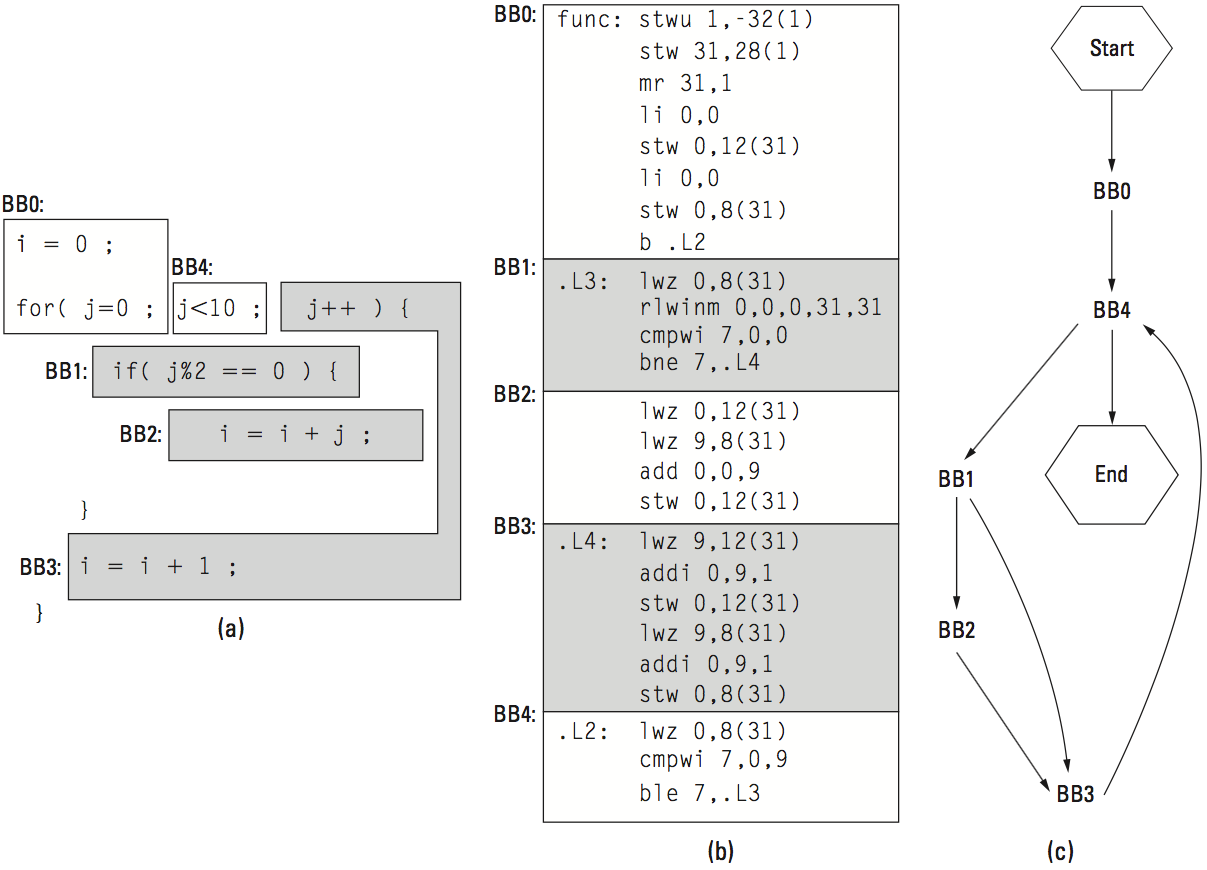
\includegraphics[width=0.35\textwidth]{img/f3-6.png}
         \caption{Identificação de blocos básicos e a representação por meio de um grafo não atrelado à uma especificação \hs.}
         \label{fig:f3-6}
      \end{figure}
      \end{comment}

      \todo{colocar isso num lugar melhro?}
      A decomposição de um DRS pode gerar dois componentes: uma porção a ser realizada em \hardware\ e; outra executada em \software.
      Essa decisão de divisão é chamada de Problema de Particionamento.
      Segundo \cite{Sass2010}, para sistemas em FPGA, o particionamento é um sub-problema de um problema mais geral no âmbito de \codesign, onde refere-se ao \design\ cooperativo entre engenheiros de \hs\ para um desenvolvimento mais eficiente.% envolvendo \textit{stakeholders}, por exemplo.
      %Para continuar, deve-se definir alguns conceitos básicos, descritos na Seção \ref{sec:gc}.

      %\subsubsection{Grafo de Chamada}
      \label{sec:gc}
         %Modelado uma sub-rotina de um DRS utilizando o GCF, definido na Seção \ref{sec:GCF}, agora será descrito uma nova notação, chamada de Grafo de Chamada (GC) utilizado para o entendimento da partição.
         Um Grafo de Chamada (GF) consiste num conjunto de GCFs, um por sub-rotinas, ou seja, $\mathcal{C} = {C_0, C_1, \dots C_{n-1}}$
         %
         %\begin{equation}
         %   \mathcal{C} = {C_0, C_1, \dots C_{n-1}}
         %\end{equation}
         %
         %onde $ C_i = (V_i, E_i) $
         onde $ C_i = (B_i, F_i) $ representa o GCF de uma sub-rotina $ i $. %, como mostrado na Equação~\ref{eq:subrotina}.
         Sendo assim, o grafo estático de chamada da aplicação é escrito por $\mathcal{A} = (\mathcal{C}, \mathcal{L}) \label{eq:a}$
         %
         %\begin{equation}
         %   \mathcal{A} = (\mathcal{C}, \mathcal{L}) \label{eq:a}
         %\end{equation}
         %
         onde \A\ representa uma aplicação específica e $ \mathcal{L} \subseteq \mathcal{C} \times \mathcal{C} $ é um subconjunto do plano cartesiano dos GCF.
         Duas sub-rotinas são relacionadas se podem ser determinadas que, no tempo de compilação, a sub-rotina $ i $ tem potencial de invocar a sub-rotina $ j $, ou seja, $ (C_i, C_j) \in \mathcal{L} $.

         %É assumido que os blocos básicos de cada sub-rotina são disjuntos, ou seja, cada bloco básico em uma aplicação pertence a exatamente um GCF.
         %Além do mais, é assumido também que um nó raiz para o GC é implícito, ou seja, uma sub-rotina é designada a iniciar a execução.
         %Nem todos os executáveis podem ser expressados nesse modelo.
         %Por exemplo, o manuseio de sinais e interrupções não são representadas e assim, não é possível determinar todos vértices $ F_i $ em uma dada sub-rotina $ C_i $ de um GCF antes da execução.
         %Uma outra forma é com o paradigma de orientação à objeto.
         %Ele depende do tempo de execução para conectar os métodos virtuais invocados e dessa forma, por \design, esse paradigma nos previne de saber todos os vértices antes da execução.
         %Para agora, será considerado que o modelo é suficiente para ser expressado em \design\ referencial de \software.

         %Um equívoco comum é de que uma definição formal de particionamento só aplica à separação de aplicação componentes de \hs, ou seja, a partição contém exatamente dois conjuntos.
         %Todavia, para fazer o problema mais tratável, é comum agrupar primeiramente operandos em recursos, ou seja, uma partição com um grande número de subconjuntos, e então mapeia esses recursos tanto em \hardware\ quanto \software.
         %Assumindo que esses recursos atuam razoavelmente bem \textit{clustered}, então a decomposição de uma aplicação em componentes de \hs\ pode ser dirigida por comparações de ganho de performance desse recurso contra outro situado no outro conjunto.

         %Definidos os conceitos prévios, será definido agora, formalmente, o conceito de uma partição.

         Com esses conceitos definidos, uma partição $ \mathcal{S} = \{S_0, S_1, \dots\} $ de um conjunto universal $ U $ é um conjunto de subconjuntos de $ U $ sendo que
         %
         \begin{gather}
            \bigcup_{S \in \mathcal{S}} S = U \label{eq:part_form_1}\\
            \forall S, S' \in \mathcal{S} | S \cap S' = \emptyset \label{eq:part_form_2}\\
            \forall S \in \mathcal{S} | \mathcal{S} \cdot S \neq \emptyset \label{eq:part_form_3}
         \end{gather}
         %
         onde a Equação~\ref{eq:part_form_1} diz que cada elemento de $ U $ é um membro de, pelo menos, um subconjunto $ S \in \mathcal{S} $, e as Equações~\ref{eq:part_form_2} e \ref{eq:part_form_3} que os subconjuntos $ S \in \mathcal{S} $ são emparelhados disjuntos e não vazio.
         Em outras palavras, cada elemento do nosso universo $ U $ termina exatamente em um dos subconjuntos de $\mathcal{S}$ e nenhum dos subconjuntos são vazios.

         Com isso é possível aplicar o formalismo à $ \mathcal{A} $ se assumirmos que nosso universo é o conjunto de todos os blocos $B$ de todas as sub-rotinas de um dispositivo \wearable, então $U$ é as partições de sub-rotinas
         %
         \begin{equation}
            U = \bigcup_{C \in \mathcal{C}} B(C) \label{eq:bigcup}
         \end{equation}
         %
         e chamaremos de partição natural da aplicação, onde
         %
         \begin{equation} \small
            \mathcal{S}  = \left \{
            \underbrace{\left \{ b_0, b_1, \dots, b_{i-1} \right \}}_{\textnormal{sub-rotina }C_0},
            \underbrace{\left \{ b_i, b_{i+1}, \dots \right \}}_{\textnormal{sub-rotina }C_1},\dots
            \underbrace{\left \{ b_j, b_{j+1}, \dots \right \}}_{\textnormal{sub-rotina }C_{n-1}}
            \right \}
         \end{equation}


          \makeatletter
          \def\@eqnnum{{\normalsize \normalcolor (\theequation)}}
           \makeatother

         %
         O propósito é reorganizar a partição de blocos básicos e então mapear cada subconjunto de ambos os \hs.
         Dessa forma, pode-se criar e remover subconjuntos não vazios, e mover blocos básicos ao redor até termos uma nova partição e assim termos um novo resultado $ \mathcal{A}’ = (\mathcal{C}’, \mathcal{L}’) $, inferido a partir da reorganização da partição $ \mathcal{X}’ $.
         O segundo passo é mapear cada subconjunto de $ \mathcal{X} $ para ambos \hs\ como é exibido abaixo

         { \small
         \begin{equation}
            \mathcal{X}'\!=\!\left \{
            \underbrace{
               \underbrace{
                  \left \{ b_0, b_1, ..., b_{i-1} \right \}
               }_{\textnormal{sub-rotina }C_0}
               ...
               \underbrace{
                  \left \{ b_j, b_{j+1}, ... \right \}
               }_{\textnormal{sub-rotina }C_{n-i}}
               ...
            }_{\textnormal{\software}}
            %\
            \underbrace{
               \underbrace{
                  \left \{ b_i, b_{i+1}, ... \right \}
               }_{\textnormal{sub-rotina }C_{n-1}}
               ...
            }_{\textnormal{\hardware}}
            \right \} \label{eq:part_final}
         \end{equation}
         }

         A seguir será explicado como a performance pode ser utilizada para guiar o particionamento.
         %Para explicar como performance pode ser utilizada para guiar o particionamento, será descrita uma métrica simples chamada taxa de execução\footnote{Taxa de execução é a velocidade na qual um sistema computacional completa uma aplicação, e em um sistema de plataforma FPGA olhamos também para o \hardware\ para melhorar sua taxa de execução.} a seguir.


   \subsection{Análise para Ganho de Performance} \label{sec:ganho_performance}
      %É parcialmente motivada pelo fato de que: \textit{a)} o ganho de performance é relativamente fácil de ser mensurado e \textit{b)} por causa de que, de todas as métricas comumente utilizadas, \speedup\ é frequentemente a mais importante.
      Diferente do mundo \software\ onde se tem análise de ordem de complexidade, em \hardware\ não possui-se um guia geral para comparação.
      O ganho de performance para aplicações em geral pode estar na acumulação de pequenos ganhos.% que deveriam ser perdido numa aplicação direta na teoria de complexidade.

      % tempo software
      Para o \software, será usado a informação de \profile\ para coletar o tempo total de execução, bem com uma fração do tempo gasto em cada sub-rotina.
      %O produto disso é a aproximação entre o tempo necessário para executar uma porção de aplicação em \software\ e usar isso como o tempo que se espera que tomará em futuras execuções.
      %É considerado uma aproximação pois é dependente dos conjuntos de dados de entrada para muitas aplicações além da existência de erros que podem impactar a performance.
      Será utilizado $ s(i) $ para representar o tempo de execução esperado para uma invocação de uma sub-rotina $ i $.

      % tempo hardware
      Precisa-se também aproximar o tempo que uma implementação equivalente em \hardware\ que iria tomar e que, em \hardware, isso é frequentemente mais preciso.
      Pra isso, uma ferramenta \textit{profiling} auxiliar à síntese poderá dar uma aproximação de acurácia de propagação de tempo.
      %Ou, se o recurso é \textit{pipelined}, o número de estágios é mais precisamente conhecido.
      %Caso o recurso inclua controle de fluxo mas não contenha nenhum \textit{loop}, pode-se considerar o caminho mais longo como uma estimativa conservativa.
      %Recursos com um número variável de iterações através de um \textit{loop} apresentam o maior obstáculo para encontrar um tempo de \hardware\ aproximado.
      %Nesse caso, implementação e \textit{profiling} com recurso em \hardware\ pode ser a única solução.
      Independente, assume-se que uma aproximação apropriada $ h(i) $ para o existente tempo de execução em \hardware, sendo $ i $ o módulo construído.

      % tempo mudanca de estado, configuracao, latencia
      Por fim, a `interfaceação' entre \hs\ requer tempo e este custo também precisa ser contabilizado.
      Pode-se aproximar deste custo pela aproximação do montante total do estado que necessita ser transferido ou o custo de configuração e latência.
      Em ambos os caso, são representados por $ m(i) $ para recursos $ i \in \mathcal{H} $, sendo $\mathcal{H}$ o conjunto de recursos do \hardware.

      % y é speedup
      Por fim, o ganho, ao comparar uma solução \hs\ contra uma solução puramente \software, é tipicamente mensurado como \speedup, Equação~\ref{eq:speedup1}.
      Utiliza-se $ \gamma $ para sua representação, permitindo comparar recursos diferentes contra outros para determinar melhores particionamentos.
      Qualquer subconjunto de blocos que não produzem um maior ganho de performance, podem ser desconsiderados, ou seja, somente $ \gamma > 1.0 $ são considerados recursos candidatos.
      %Então quando considerado se um conjunto particular de blocos básicos deveriam ser mapeados ao \hardware\ ou \software, estamos interessados em seu ganho em \speedup, ou seja
      %
      \begin{equation}
         \gamma =
         \frac{
            \textnormal{\textit{hardware speed}}
         }{
            \textnormal{\textit{software speed}}
         }
         =
         \frac{
            \frac{
               1
            } {
               \textnormal{\textit{hardware time}}
            }
         } {
            \frac{
               1
            }{
               \textnormal{\textit{software time}}
            }
         }
         =
         \frac{
            \textnormal{\textit{software time}}
         } {
            \textnormal{\textit{hardware time}}
         } \label{eq:speedup1}
      \end{equation}
      %
      Mais especificamente, interessa-se no ganho de performance individual de cada recurso e assim, definindo $ \gamma(i), i \in \mathcal{C} $
      %
      \begin{equation}
         \gamma(i) = \frac{s(i)}{h(i) + m(i)}
      \end{equation}
      %
      %onde $ h(i) $ e $ s(i) $ são o tempo de execução de uma implementação de um recurso $ i $ em \hs\ e a função $ m(i) $ é o tempo que se leva para sincronização, ou seja, o tempo que leva para guiar um dado entre o processador e o item reconfigurável.

      %Assumindo por um momento que usaremos esse recurso separado em nosso \design, deve-se questionar sobre o quão rápido é a aplicação.
      A velocidade da aplicação é dependente dos ganhos de performance do recurso e o quão frequentemente ele é utilizado no DRS.
      Pode-se ter essa fração do tempo gerado de um recurso particular $ p(i) $ a partir de informações de \textit{profile} e dessa forma o \speedup\ da aplicação no geral será
      %
      \begin{equation}
         \Gamma = \left [
         (1 - p(i))
         +
         \frac{
            p(i)
         }{
            \gamma(i)
         } \right ]^{-1}
      \end{equation}
      %
      A inversão representa que estamos movendo entre taxa de execução e tempo de execução para manter o sentido de ganho de performance.

      %A partir dessa equação, podemos observar que aumentando a velocidade do \hardware\ de um único recurso tem-se menos e menos impacto na performance da aplicação a medida que sua frequência decresce.

      %Para aumentar a performance sistêmica de uma aplicação no geral, também deve-se aumentar o sistema com múltiplos recursos que aumentará a performance de componentes individualmente assim como aumentando a fração agregada de tempo gasto em \hardware.
      Para computar o \speedup\ de múltiplos recursos em \hardware, deve-se avaliar o ganho sistêmico de um conjunto de recursos $ \mathbb{D} $.
      %Para estimar a performance desta partição, podemos adicionar recursos e rearranjar os termos para ter um ganho de performance almejado no geral,
      Assim, para o cálculo de performance dos recursos, utiliza-se da Equação \ref{eq:d_final}.
      %
      \begin{equation}
         \Gamma (\mathbb{D}) =
         \left [
         \sum _{i \in \mathbb{D}} \left (
         \frac{
            p(i)
         }{
            \gamma(i)
         }-p(i)
         \right) + 1
         \right ]^{-1} \label{eq:d_final}
      \end{equation}

      \subsubsection{A Considerações de Recursos Finitos em Componentes Eletrônicos} \label{sec:recursos}

         Uma hipótese de consideração de recursos seria adicionar esses na abordagem $\sum_i p_i$, ou seja, implementar tudo em \hardware\ para maximizar a performance, o que no caso, ignoraria todos os custos de desenvolvimento e recursos finitos.
         Entretanto, num FPGA, há um número finito de recursos disponíveis para sintetização de circuitos em \hardware\ e como tais recursos são limitados, a maioria das aplicações realísticas iriam exceder esse limite disponível. \todo{aqui entra o fpga de pequeno porte}

         Uma outra forma é contar o número de células lógicas requeridas para cada recurso.
         Um FPGA que terá um valor total escalar $ r_{FPGA} $, representará o total de números de células lógicas disponíveis para sintetização.
         Então $ r(i) $ pode ser usado para representar a quantidade de células lógicas requeridas por cada recurso $ i $.
         Fazendo uma simples relação, tem-se que $ \sum_{i \in \mathbb{D}} r(i) < r_{FPGA} $ restringe quão largo $ \mathbb{D} $ pode crescer, onde $ \mathbb{D} $ é o conjunto de recurso incluídos no \design.

         Sabendo que dispositivos modernos são heterogêneos, uma típica plataforma FPGA tem múltiplos tipos de recursos além de células lógicas como memória, blocos DSP, etc., podendo ser representados por um vetor de recursos
         %
         \begin{equation} \small
            \vec{r}_{FPGA} =
            \begin{pmatrix}
            r_{Logic\ Cells} \\
            r_{Memory}\\
            r_{DSP}\\
            \vdots \\
            r_{n-1}
            \end{pmatrix}
         \end{equation}
         %
         e com isso,
         %
         %\begin{equation}
            $\sum_{i \in \mathbb{D}} \vec{r}(i) < \vec{r}_{FPGA}$.
         %\end{equation}
         %

         %Infelizmente\todo{a}, esse modelo não leva em consideração o fato de que alguns recursos alocados podem interferir em outros, além de que a estimativa de performance é frequentemente baseada na suposição que recursos são próximos um do outro e recursos de rotas não são parte integral do modelo.


%%!TEX root = ../main.tex
% !TeX encoding = UTF-8
%\chapter{O Particionamento de \HS\ para Sistemas \Wearables} \label{chap:desenvolvimento}
   \section{O Particionamento de Hardware e Software para Sistemas Wearables} \label{sec:desenvolvimento}

      %De início, será considerado como aplicaçãåo \wearable\ um conjunto de instruções organizadas, e como visto na Seção \ref{sec:gc}, esta também representada por uma coleção de grafos de controle de fluxo, ou seja, GC, especificando a sua ordem de execução.
      A partir deste, será feito análises a fim da procura de um particionamento que atenda aos requisitos de dispositivos \wearables\ como poder de processamento sem o \textit{trade-off} de energia, além de miniaturização, confiabilidade e outros.

      %Após esclarecidos algumas definições prévias (Seção~\ref{sec:definicoes_previas}), será apresentado o problema na Seção~\ref{sec:declaracao_problema}.
      %Alguns fatores podem ajudar nas decisões de particionamento tal como expectativa de ganho de performance (Seção \ref{sec:ganho_performance}) e os recursos utilizados em \hardware\ (Seção \ref{sec:recursos}).%, a forma na qual são usados e, talvez os mais importantes, quanto de sobrecarga de comunicação a decomposição impõe (Seção \ref{sec:comunicacao}) \todo{deixar?}e dificuldade de implementar um conjunto específico em \hardware\ (Seção \ref{sec:dificuldades}).\todo{organizar}


   \subsection{Declaração do Problema} \label{sec:declaracao_problema}
      %Nesta seção serão apresentadas as declarações matemáticas do problema de agrupamento de instruções em recursos e seus mapeamentos em \hardware\ ou \software, ou seja, o particionamento \hs.
      %Segundo \cite{Sass2010}, a forma mais comum de transcrever é descrever manualmente o \core\ com um HDL utilizando \design\ referencial de \software\ como especificação, método utilizado para descrever o problema.

      No particionamento, muitos problemas práticos impactam diretamente na performance do sistema.
      Nem todos os problemas podem ser incorporados num modelo analítico \cite{Wang2016}, e por isso, só podemos esperar que as soluções matemáticas produzam uma resposta aproximada ao problema de particionamento ao utilizar a declaração formal, pois muitas das entradas do modelo são estimadas ou aproximações no qual futuramente degrada a fidelidade de resultados.
      %%Este é um fato relevante pois com isso, resolvendo o problema de particionamento `no papel', tem-se um particionamento que é próximo ao ótimo.
      %%Assim, cabe ao \designer\ ser habilidoso em usar os guias e projetar uma solução mais refinada.
      Dessa forma, é mais eficiente usar uma combinação de técnicas \textit{ad hoc} e matemáticas para encontrar uma solução ótima ou aproximada como será feito, do que simplesmente confiar numa intuição.


      %\begin{comment}
      %\subsection{Declaração do Problema}
      %Já descrito as ferramentas matemáticas necessárias para descrever o problema fundamental do particionamento no Capítulo \ref{chap:revisao_bibliografica}, pode-se então descrever formalmente o problema em termos de variáveis. % e descrever um algoritmo \todo{algorit?}para encontrar uma solução aproximada.
      %
      %A ideia básica consiste em encontrar um particionamento para todos os blocos básicos de uma aplicação e então separá-los em \hs.
      Formalmente, procura-se por uma partição $ \mathcal{P} $ de todos os blocos $ U $ de uma aplicação.
      %
      %$$ U = \bigcup_{C \in \mathcal{C}} B(C) $$
      %
      %$ C = (B,F) $
      Definida a partição e o universo, tem-se então um subconjunto $ \mathbb{C}\ |\ \mathbb{C} \subseteq U $, onde $ C \in \mathcal{C} $ é um vértice de um $ \mathcal{A} = (\mathcal{C}, \mathcal{L}) $.
      O conjunto $ \mathbb{C} $, chamado conjunto de candidatos, contém todos os recursos arquiteturais potenciais, ou seja, o subconjunto de $ U $ que é esperado para melhorar a performance do sistema se implementado em um \hardware\ reconfigurável.
      Devido ao limite de recursos, deve-se refinar para o subconjunto $ \mathbb{D} \subseteq \mathbb{C} $ que maximiza nosso métrica de performance.
      Assim, tem-se
      \begin{equation}
         \begin{array}{rrcl}
         \textnormal{max}                 & \Gamma ( \mathbb{D})               & ~   & ~                \\
         subject\ to & \sum_{i \in \mathbb{D}} \vec{r}(i) & < & \vec{r}_{FPGA}
         \end{array}
         \label{eq:constraints}
      \end{equation}
      %
      %Descrevendo isso algoritmicamente, uma abordagem seria encontrar todas as partições de $ U $, sintetizando e \textit{profiling} cada partição, e então, quantitativamente avaliar cada $ \Gamma $.
      %Entretanto, este é um problema linear inteiro devido à natureza de alocação e utilização dos recurso físicos do FPGA. %(Seção \ref{sec:pli})

      A seguir, será descrito como é feito uma abordagem para tal, seguindo estudos de \cite{Arato2003, Wang2016}.


   %\subsection{Metodologia Proposta}
   \subsection{Proposta do Procedimento Analítico} \label{sec:proposta}

      Neste, apresenta-se o algoritmo e sua descrição classificadas por cada fim a ser alcançado.
      %Neste, será formulada uma proposta de metodologia analítica baseada nos conceitos propostos pela literatura, com o foco em componentes procedurais integrados à sistemas \wearables.
      %E com isso, o trabalho consiste em desenvolver seus respectivos grafos e realizar o particionamento a fim de encontrar uma solução aproximada, respeitando os seus requisitos de funcionamento.
      %
      %Tal metodologia, apresentada pelo Algoritmo~\ref{alg:proposta}, será considerada apenas como uma orientação para os passos a serem realizados, sendo então, uma proposta representativa do processo a ser realizado para a análise e decisão de particionamento.

      \begin{algorithm}[!ht] \footnotesize
         \SetKwData{itt}{it}
         \SetKwData{pl}{partition\_list}
         \SetKwData{complexSet}{how\_complex\_set\_is}
         \SetKwData{md}{matriz\_dados}
         \SetKwData{complexSet}{how\_complex\_set\_is}
         \SetKwFunction{graph}{make\_graph}
         \SetKwFunction{porte}{analyse\_complex\_set}
         \SetKwFunction{synth}{synthesize}
         \SetKwFunction{resources}{resources\_used}
         \SetKwFunction{die}{die\_used}
         \SetKwFunction{energy}{energy\_spent}
         \SetKwFunction{profiling}{profile}
         \SetKwFunction{performance}{performance\_analysis}
         \SetKwFunction{factor}{complexity\_factor}
         \SetKwFunction{ilp}{integer\_linear\_solve}
         \SetKwFunction{heuristic}{heuristic}
         \KwIn{a project description.}
         \KwOut{a partition solved.}

         %\BlankLine
         \Begin{

            \BlankLine
            \func{profiling}();
            \BlankLine

            %\tcp{extration project analyses}
            %\graph{Flow Control Graph}\;
            %\graph{Call Graph}\;
            %\complexSet $\leftarrow$ \porte{}\tcp*{verify if it is a big project}

            \BlankLine

            \If{exist partitions that can be synthesized}{
               \ForEach{partition project:\vars{it} $\in$ \vars{partition\_list}}{
                  \func{synth}(\vars{it});
                  \BlankLine
                  \func{resources}(\vars{it})\tcp*{analysis after synth}
                  \func{die}(\vars{it})\;
                  \func{energy}(\vars{it});
                  %\BlankLine


                  \func{performance}(\vars{it});
               }
               \BlankLine

               %\uIf(\tcp*[f]{verify if it is a small project}){\factor{\complexSet}}{
                  \func{ilp}(\vars{partition\_list})\tcp*{analyse quantitatively each $ \Gamma $}
               %}
               %\lElse{
                  %\heuristic{\vars{partition\_list})\;
               %}
            }
         }
         \caption{Metodologia de avaliação de \wearables.}
         \label{alg:proposta}
      \end{algorithm}
        \todo[inline]{atualizar}
        \todo[inline]{melhorar}
      %Apresentado o procedimento metodológico, a seguir será listada cada função pertencente à metodologia acima, descrevendo suas funções e seu propósito no trabalho para a obtenção dos objetivos.
      %Para um melhor compreendimento, serão divididos em quatro seções, sendo elas: visualização do projeto, síntese, análise de síntese, particionamento.

      \begin{enumerate}
         \item Procedimentos para visualização geral do projeto.
         %Por meio dos dados do \profile\ e a construção dos grafos, é possível ter uma visão geral, verificando se o sistema possui possíveis seções de processamentos críticos para a realização de particionamento \hs.

         \begin{itemize}
            \item \texttt{profile():}
               procedimento referente à Seção~\ref{sec:profile}.
               %Realiza-se uma análise de tempo gasto em cada procedimento do projeto, apresentando-a ao final de sua execução.
               %Com os resultados, é possível ver locais onde existe um tempo maior de processamento gasto ou de recursos utilizados indicando uma verificação detalhada sobre este a fim de candidatá-lo para uma implementação em \hardware;

               \begin{comment}
            \item \texttt{make\_graph(}\textit{type}\texttt{):}
               constroi-se grafos relativos ao projeto, sendo estes de acordo com o tipo especificado no parâmetro.
               %A construção do grafo segue como descrito na Seção~\ref{sec:GCF} na qual procura-se por seções de códigos compondo-os em blocos, compreendendo o fluxo do algoritmo e consecutivamente os procedimentos de chamadas.
               O parâmetro simboliza a especificação de qual tipo de grafo será construído, sendo ele um GCF (Seção~\ref{sec:GCF}) ou GC (Seção~\ref{sec:gc}), que como já explicado, necessita do anterior para sua construção;
            \end{comment}
         \end{itemize}

         \item Procedimento de síntese.
         \begin{itemize}
            \item \texttt{synthesize():}
               caso exista uma possibilidade de particionamento,
               %análise obtida pelo \profile, visualização do grafo e obtenção de uma lista de candidatos,
               realiza-se então o procedimento de geração de HDL para o desenvolvimento de aceleradores em \textit{hardware} reconfigurável.% e sua análise de performance e gastos tanto de energia quanto de recursos;
         \end{itemize}

         \item Após a execução do processo de síntese, é possível obter vários dados analíticos de alocação de recursos. % como quantidade de elementos lógicos utilizados, pinos virtuais e físicos, quantidade de bits de memória, além de vários outros.
         %E com a sua sintetização na plataforma, também é possível obter a avaliação de consumo energético, \profile\ e performance.
         Estes são representados pelos métodos abaixo na qual, aplica-se a cada componente sintetizado separadamente.
         \begin{itemize}
            \item \texttt{resources\_used():}
               quais e a quantidade de recursos alocados para utilização no projeto de geração de aceleradores;
               %A alocação de muitos recursos implica num gasto maior de energia criando um \textit{trade-off} a ser analisado;

            \item \texttt{die\_used():}
               tamanho do \textit{die} utilizado para o projeto do acelerador.
               %Sistemas \wearables\ possuem como requisito a sua miniaturização, impedindo que seu uso limite a capacidade de locomoção, usabilidade ou conforto do usuário, por exemplo;

            \item \texttt{energy\_spent():}
               estimação de valores energéticos do uso do recurso implementado.%, incluindo os módulos pertencentes a ele como memórias, DSPs e quaisquer outros que estejam integrados à plataforma;

            \item \texttt{performance\_analysis():}
               comparação das implementações em \hardware\ sobre os recursos em nível de \textit{software}, ou seja, análise de performance.
         \end{itemize}

         \item Procedimento de escolha de particionamento.
         \begin{itemize}
            \item \texttt{integer\_linear\_solver():}
               após realizado todas as análises individuais acima, inicia-se o processo de procura de uma solução de particionamento que obtenha bons resultados nos requisitos de um sistema \wearable.
               %Dessa forma, é realizado uma avaliação por meio de um \textit{solver} linear inteiro segundo os dados obtidos.
               %Com o \textit{solver}, é possível realizar uma busca a procura de um particionamento que atenda a quantidade máxima de restrições exigidas por um \wearable.
         \end{itemize}
      \end{enumerate}


      %Conclusão
      Assim, o trabalho consiste numa metodologia na qual aborda o particionamento para dispositivos \wearables, partindo de uma análise de execução do \software, candidatando alguns procedimentos para sua sintetização e assim a avaliação destes segundo os recursos utilizados para a completude de suas tarefas o que chamamos de particionamento, consistindo da procura de um conjunto que traga melhor desempenho no seu uso.
      Tudo isso, utilizando recursos disponibilizados pela plataforma em \hardware.
      %O Algoritmo~\ref{alg:proposta} tem como o objetivo a demonstração do passos necessários para o compreendimento do sistema a ser analisado e consecutivamente a sua partição em busca do aprimoramento da sua performance.


%%!TEX root = ../main.tex
% !TeX encoding = UTF-8
\section{Experimentos}

    \subsection{Capacete para Segurança de Ciclistas}
        Desenvolveu-se um protótipo de capacete na qual realiza-se verificações de distância de objetos nas costas do ciclista a fim de alertá-lo de possíveis riscos de acidentes.
        Caso esteja em situação de risco, o capacete emitirá sinais visuais luminosos, além do envio de aviso para um segundo dispositivo avisando de sua situação sendo este não fazendo parte do trabalho.
        Para dados mais coerentes com a distância real, construiu-se um capacete modular a fim de fazer diferentes testes sendo então, com 1 à 3 sensores de distância além de um \buffer\ de dados de tamanho 5, 10 e 15 para processamento das distâncias de cada sensor, discutidos a seguir.
        
        \begin{figure}[h] \centering
            \vspace{-0.5em}
            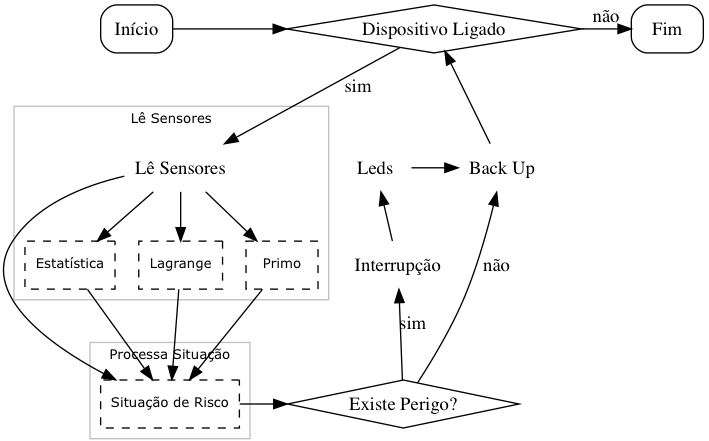
\includegraphics[width=0.48\textwidth]{img/capacete.png}
            \caption{Grafo de chamada do algoritmo base do \wearable.}
            \label{fig:gc}
        \end{figure}
        
        Como é exibido na Figura \ref{fig:gc}, os passos do \wearable\ constituem-se basicamente de leitura das distâncias, cálculo de risco e aviso ao usuário.
        O particionamento será avaliado em duas seções principais, sendo elas a de leitura e de processo de situações, constituindo de 4 situações diferentes de particionamento para análise.
        Na seção de leitura de sensores, serão adicionados: \textit{1)} algoritmo de análise estatística (Algoritmo \ref{alg:statistic}) na qual calculará valores de desvio padrão e variância dos valores no \buffer; \textit{2)} algoritmo de lagrange (Algoritmo \ref{alg:lagrange}) interpolará novas distâncias e; \textit{3)} algoritmo de números primos (Algoritmo \ref{alg:prime}) avaliará se a soma das distâncias lidas correspondem à números primos.
        A análise serão feitas por meio de exclusão, selecionando apenas um algoritmo por vez e adicionado ao código para análise.
        Quando nenhum desta seção for utilizado para particionamento, utiliza-se então: \textit{4)} algoritmo de processamento de risco (Algoritmo \ref{alg:risk}), na seção de processo de situações.
        Este por sua vez está em todas as análises, pois é passo necessário para a iteração do \wearable.
        
    
        A placa utilizada para sintetização foi uma Arty A7-35T.% com 32 mil elementos lógicos e \textit{clock} de 450MHz.
        Utilizou-se o sistema \textit{soft-processor} MicroBlaze para processamento do código em \software.
        Todos os algoritmos foram construídos utilizando ferramenta HLS \todo{sigla} e incorporados ao projeto base.
        A comunicação entre \hs\ é feita utilizando interface AXI.
        A medição de distância é realizada com um sensor ultrassônico e a comunicação com o segundo dispositivo utiliza \textit{Bluetooth Low Energy}.
        
        
    \subsection{Testes Realizados}
        % Explicando os testes
        Para a realização dos testes, será feito um procedimento tendo base a Figura \ref{fig:distance}. 
        O teste possui 2 passos, a aproximação e o distanciamento de objeto, na qual serão aplicados no decorrer de 12 iterações do \wearable.
        %
        \textit{Iteração 1:} o ciclista encontra-se a uma distância de 130 centímetros do objeto, sendo sua situação declarada como Segura;
        %
        \textit{Iteração 4:} o objeto inicia um movimento de aproximação ao ciclista chegando a ultrapassar o limite mínimo de 30 centímetros iniciando a situação de Risco;
        %
        \textit{Iteração 9:} o objeto afasta novamente do ciclista para 130 centímetros, retornando à situação Segura.
        Tanto o movimento de aproximação quanto o de afastamento são feitos manualmente para que simule de fato a situação real de um ciclista em seu meio;
        \textit{Iteração 12:} última leitura para testes.
        %
        Sendo assim, cada algoritmo será performa e separadamente analisados em ambos os níveis de \software\ e \hardware.
        Para uma análise estatística dos resultados, esse conjunto de 12 iterações e os respectivos movimentos repetirão por 30 vezes.

        \begin{figure}[h] \centering
            \vspace{-1em}
            
\includegraphics[width=0.5\textwidth]{img/distance.png}
            \caption{Testes de resposta do \wearable\ à situações de possível perigo.}
            \label{fig:distance}
        \end{figure}

\section{Resultados}
    % tabela hls
    Os recursos utilizados em cada algoritmo ao realizar o seu particionamento é exibido na Tabela \ref{tab:hls}.
    \begin{table}[h]\centering
        \vspace{-1em}
        \scriptsize
        %\raaa{1.0}
        \raaa{0.9}
        \caption{Recursos Utilizados no HLS.}
        \begin{tabular}{rrr|rr|rr|rr||rr}
            \toprule
            &\multicolumn{2}{c}{Expressões} & \multicolumn{2}{c}{Instâncias}      & \multicolumn{2}{c}{Multiplex}  & \multicolumn{2}{c}{Regist.} & \multicolumn{2}{c}{\textit{Total}} \\
            \cmidrule{2-11}
            %\cmidrule{2-3} \cmidrule{5-6} \cmidrule{8-9} \cmidrule{11-12} \cmidrule{14-15}
            & \textit{Lut} & \textit{Ff} & \textit{Lut} & \textit{Ff} & \textit{Lut} & \textit{Ff} & \textit{Lut} & \textit{Ff} & \textit{Lut} & \textit{Ff} \\
            \midrule
            \A$_1$&52 & 0     & 1948 & 1474   & 364 & 0      & 0 & 394   & 2364 & 1868 \\ 
            \A$_2$&128 & 0    & 2048 & 1425   & 309 & 0      & 0 & 479   & 2483 & 1904 \\ 
            \A$_3$&1826 & 0   & 486 & 552     & 236 & 0      & 0 & 527   & 2448 & 1079 \\ 
            \A$_4$&18 & 0     & 120  & 82     & 15  & 0      & 0 & 34    & 153  & 116  \\ 
            \bottomrule
        \end{tabular}
        \label{tab:hls}
    \end{table}

    % tabela vivado
    Ao adicionar o algoritmo em \hardware\ ao projeto base é possível calcular seu gasto de recursos bem como seu gasto energético.
    Tais valores são exibidos na Tablea \ref{tab:vivado}.
    \todo[inline]{parei aqui}
    \begin{table}[h]\centering
        \vspace{-1em}
        \scriptsize
        %\raaa{1.0}
        \raaa{0.9}
        \caption{Recursos Utilizados no Projeto Final.}
        \begin{tabular}{rcccccc}
            \toprule
            %&\multicolumn{2}{c}{Expressões} & \multicolumn{2}{c}{Instâncias}      & \multicolumn{2}{c}{Multiplex}  & \multicolumn{2}{c}{Regist.} & \multicolumn{2}{c}{\textit{Total}} \\
            %\cmidrule{2-11}
            %\cmidrule{2-3} \cmidrule{5-6} \cmidrule{8-9} \cmidrule{11-12} \cmidrule{14-15}
            & LUT    & LUTRAM   & FF     & I/O     & On-Chip Power & Off-ChipPower \\
            \cmidrule{2-7}
            
                  & 20800  & 9600     & 41600  & 210    & -              & -      \\
            \A$_1$& 13640  & 1822     & 13080  & 104    & 0,972W         & 0,506W \\ 
            \A$_2$& 13502  & 1808     & 13193  & 104    & 0,968W         & 0,506W \\ 
            \A$_3$& 12959  & 1782     & 12559  & 104    & 0,933W         & 0,506W \\
            \A$_4$& 12109  & 1781     & 11742  & 104    & 0,929W         & 0,506W \\ 
            \bottomrule
        \end{tabular}
        \label{tab:vivado}
    \end{table}

    %tabela ms
    A Tabela~\ref{tab:iterations} exibe os valores obtidos da análise de performance comparando os sistemas em \software\ e \hardware. 
    Valores exibidos mostram a diferença performática de \software\ e \hardware\ sendo que os valores positivos indicam o tempo na qual o algoritmo \A$_i$ obteve maior performance em \hardware, enquanto valores negativos exibem maior performance em \software, todos em milissegundos.
    As informações exibidas foram filtradas, eliminando o tempo médio gasto da atuação dos sensores bem como o tempo de envio para o dispositivo externo, ambos dependente de sua tecnologia.

    \begin{table}[h]\centering
        \vspace{-1em}
        \scriptsize
        %\raaa{1.0}
        \raaa{0.9}
        \caption{Recursos Utilizados no HLS.}
        \begin{tabular}{@{}crrr|rrr|rrr@{}}\toprule
            & \multicolumn{3}{c}{1 Sensor} & \multicolumn{3}{c}{2 Sensores} & \multicolumn{3}{c}{3 Sensores}\\
            \cmidrule{2-10}
            %\cmidrule{2-4} \cmidrule{6-8} \cmidrule{10-12} \textit{} 
            & \textit{b}:\,5 & \textit{b}:\,10 & \textit{b}:\,15 & \textit{b}:\,5 & \textit{b}:\,10 & \textit{b}:\,15 & \textit{b}:\,5 & \textit{b}:\,10 & \textit{b}:\,15 \\
            \midrule
            %\textit{sistêmica} \\
            %média     & ? & ? & ? & ? & ? & ? & ? & ? & ? \\
            \A$_1$   & -2.0   &    0.5  &    0.4  &   -2.7  &   -1.6  &   -1.8  &    0.4  &   0.3   &     4.2   \\
            \A$_2$   &  7.7   &    9.3  &    8.6  &   10.9  &    9.9  &   11.6  &   10.2  &   12.0  &    12.1   \\
            \A$_3$   &  2.8   &   12.2  &   91.8  &    1.6  &   44.6  &   13.9  &    4.1  &   64.8  &   231.3   \\
            \A$_4$   & 17.8   &   17.2  &   16.9  &   15.0  &   14.9  &   12.9  &   15.0  &   17.5  &    18.4   \\
            \bottomrule
        \end{tabular}
        \label{tab:iterations}
    \end{table}

    Os algoritmos \A$_i$ representam respectivamente Estatístico, Lagrange, Números primos e Risco, variando o número de sensores e o tamanho de seu \buffer\ interno.
  

\begin{comment}
    Expression & Instance      & Multiplexer  & Register & Total
    52 / 0     & 1948 / 1474   & 364 / 0      & 0 / 394   & 2364 / 1868 \\ statistic
    128 / 0    & 2048 / 1425   & 309 / 0      & 0 / 479   & 2483 / 1904 \\ lagrange
    1826 / 0   & 486 / 552     & 236 / 0      & 0 / 527   & 2448 / 1079 \\ prime
    18 / 0     & 120  / 82     & 15  / 0      & 0 / 34    & 153  / 116  \\ risk
    
    
    & LUT    & LUTRAM   & FF     & IO     & On-Chip Power & Power supplied to off-chip devices
    & 20800  & 9600     & 41600  & 210    & -             & - \\
    & 13640  & 1822     & 13080  & 104    & 0,972         & 0,506 \\ statistic
    & 13502  & 1808     & 13193  & 104    & 0,968         & 0,506 \\ lagrange
    & 12959  & 1782     & 12559  & 104    & 0,933         & 0,506 \\ prime
    & 12109  & 1781     & 11742  & 104    & 0,929         & 0,506 \\ risk
    
\end{comment}


\begin{comment}
    \begin{table}\centering
    \scriptsize
    \raaa{1.3}
    \caption{Cálculo de performance sobre variações em I/O e algoritmo particionado.}
    \begin{tabular}{@{}rrrrcrrrcrrr@{}}\toprule
    & \multicolumn{3}{c}{$\mathcal{O}(1)$} && \multicolumn{3}{c}{$\mathcal{O}(n)$} & & \multicolumn{3}{c}{$\mathcal{O}(n\log n)$}\\
    \cmidrule{2-4} \cmidrule{6-8} \cmidrule{10-12}análise& 5 & 10 & 15 && 5 & 10 & 15 &&5 & 10 & 15 \\
    \midrule \textit{sistêmica} \\
    %média     & ? & ? & ? && ? & ? & ? && ? & ? & ? \\
    $\bar{x}$     & ? & ? & ? && ? & ? & ? && ? & ? & ? \\
    $\sigma^2$ & ? & ? & ? && ? & ? & ? && ? & ? & ? \\
    $\sigma$ & ? & ? & ? && ? & ? & ? && ? & ? & ? \\
    \midrule \textit{empírica} \\
    %média     & ? & ? & ? && ? & ? & ? && ? & ? & ? \\
    $\bar{x}$     & ? & ? & ? && ? & ? & ? && ? & ? & ? \\
    $\sigma^2$ & ? & ? & ? && ? & ? & ? && ? & ? & ? \\
    $\sigma$ & ? & ? & ? && ? & ? & ? && ? & ? & ? \\
    \bottomrule
    \end{tabular}
    \end{table}
    \end{frame}
\end{comment}



%%!TEX root = ../main.tex
% !TeX encoding = UTF-8
\section{Conclusões}
   Lorem ipsum dolor sit amet, consectetur adipiscing elit. Suspendisse nisl augue, elementum ac urna ut, pretium interdum ipsum. Donec nunc tortor, sollicitudin ut dolor non, volutpat eleifend velit. Nam enim enim, lacinia sed ante eget, efficitur sodales eros. Suspendisse gravida venenatis convallis. Mauris non volutpat mauris. Nullam tempus, eros ac mollis tristique, eros mauris pellentesque odio, quis pellentesque purus lorem vel nisi. Etiam in ornare orci. Orci varius natoque penatibus et magnis dis parturient montes, nascetur ridiculus mus. Vestibulum malesuada eros felis, non mattis nunc porttitor vitae.
   
   \todo[inline]{TODO}

   Cras dictum consectetur dignissim. Curabitur porta quis est vitae luctus. Cras vitae ex faucibus, vestibulum sem mattis, varius mi. Duis cursus et elit id faucibus. Morbi tristique luctus condimentum. Curabitur quis ex sapien. In fermentum lorem nec sem viverra, ac rutrum lacus dignissim. Nam vestibulum erat id magna mollis aliquam. Nulla porttitor, eros sed scelerisque dapibus, diam ipsum congue neque, vitae malesuada augue leo tempus nisi. Ut eget gravida elit. Curabitur accumsan, ex eget mattis tempor, purus purus venenatis enim, rhoncus gravida lacus sem sed eros. Quisque finibus tellus tincidunt turpis bibendum tempus. Donec vestibulum magna lorem, vitae pellentesque justo condimentum et.

   % conference papers do not normally have an appendix
   \section*{Algoritmos Particionados}
    
    \begin{algorithm}[!ht] \footnotesize
        \KwIn{vetor buffer.}
        \KwOut{média, variância, desvio padrão.}
        
        \BlankLine
        \Begin{
            $\vars{soma}= \vars{variancia} = 0$;
            
            \For{$\func{length}(\vars{buffer})$}{$\vars{soma} \mathrel{+}= \vars{buffer}_i$;}
            
            $\vars{media} = \vars{soma} \div \func{length}(\vars{buffer})$\;
            \BlankLine
            
            
            \For{$\func{length}(\vars{buffer})$}{
                $\vars{variancia} \mathrel{+}= (\vars{buffer}_i - \vars{media})^2$\;
            }
            
            \BlankLine
            $\vars{variancia} \mathrel{\div}= \func{length}(\vars{buffer})$\;
            \BlankLine
            $\vars{dp} = \func{sqrt}(\vars{variancia})$\;
        }
        \caption{Método Estatístico.}
        \label{alg:statistic}
    \end{algorithm}
    
    
    \begin{algorithm}[!ht] \footnotesize
        \KwIn{vetor buffer, ponto.}
        \KwOut{distância interpolada.}
        
        \BlankLine
        \Begin{
            
            $\vars{nova\_distancia} = 0$\;
            
            \For{$\vars{i}\ in\ 1:\func{length}(\vars{buffer})$}{
                $\vars{c} = \vars{d} = 1$;
                
                \BlankLine
                \For{$\vars{j}\ in\ 1:\func{length}(\vars{buffer})$}{
                    \If{$\vars{i} \ne \vars{j}$}{
                        $\vars{c} \mathrel{\times}= \vars{ponto} - \vars{j}$;
                        \BlankLine
                        $\vars{d} \mathrel{\times}= \vars{i} - \vars{j}$;
                    }
                }
                \BlankLine
                $\vars{nova\_distancia} \mathrel{+}= \vars{buffer}_i \times \vars{c} \div \vars{d}$;
            }
            \BlankLine
            
            \lIf{$\vars{nova\_distancia} \ge 0$}{$\Return\ \vars{nova\_distancia}$}
            \lElse{$\Return\ 0$}
            
        }
        \caption{Método Interpolação por Lagrange.}
        \label{alg:lagrange}
    \end{algorithm}
    
    \begin{algorithm}[!ht] \footnotesize
        \KwIn{distância$_1$, distância$_2 = 0$, distância$_3 = 0$.}
        \KwOut{primaridade.}
        
        \BlankLine
        \Begin{
            
            $\vars{primo} = \vars{distancia}_1 + \vars{distancia}_2 + \vars{distancia}_3$;
            \BlankLine
            
            \lIf{$\vars{primo} \le 1$}{\Return 0}
            \BlankLine
            \lIf{$\vars{primo} = 2$}{\Return 1}
            \BlankLine
            
            \lIf{\vars{primo} $\func{mod}(2) = 0$}{$\vars{primo} \mathrel{+}= 1$}
            \BlankLine
            
            $\vars{divisor} = \vars{primo} \div 2$;
            
            \lIf{\vars{divisor} $\func{mod}(2) = 0$}{$\vars{divisor} \mathrel{+}= 1$}
            \BlankLine
            
            
            \While{\vars{divisor} $> 2$}{
                \lIf{\vars{primo} $\func{mod}(divisor) = 0$}{\Return 0}
                \BlankLine
                \vars{divisor} $\mathrel{-}= 2$;
            }
            \Return 1;
            
        }
        \caption{Método Número Primo.}
        \label{alg:prime}
    \end{algorithm}
    %
    \begin{algorithm}[!ht]
         \footnotesize
        \KwIn{distância lida; distância mínima.}
        \KwOut{boolean.}
        
        \BlankLine
        \Begin{
            \tcp{Se há risco, retorna TRUE}
            \lIf{\vars{distancia\_lida} $\le$ \vars{distancia\_minima}}{
                \Return 1
            }
            \lElse {
                \Return 0
            }
        }
        \caption{Método avaliação de Risco.}
        \label{alg:risk}
    \end{algorithm}


   % use section* for acknowledgment
   \section*{Agradecimentos}


   \todo{The authors would like to thank...}
   Agradecemos à Universidade Federal de Ouro Preto, ao CNPq e a FAPEMIG pelo subsídio dessa pesquisa.

   % trigger a \newpage just before the given reference
   % number - used to balance the columns on the last page
   % adjust value as needed - may need to be readjusted if
   % the document is modified later
   %\IEEEtriggeratref{8}
   % The "triggered" command can be changed if desired:
   %\IEEEtriggercmd{\enlargethispage{-5in}}


% references section

% can use a bibliography generated by BibTeX as a .bbl file
% BibTeX documentation can be easily obtained at:
% http://mirror.ctan.org/biblio/bibtex/contrib/doc/
% The IEEEtran BibTeX style support page is at:
% http://www.michaelshell.org/tex/ieeetran/bibtex/
\bibliographystyle{IEEEtran}
% argument is your BibTeX string definitions and bibliography database(s)
%\bibliography{IEEEabrv,bibliography}


% that's all folks
\end{document}
